\section{Results and Validation}

\subsection{Characterization of the experimental setup}

\subsubsection{Ethics and Privacy in Sensitive Data Analysis}

    The analysis of natural language in interactions with elderly users presents significant challenges regarding data privacy and ethical handling. This study implements a "Privacy by Design" approach to ensure compliance with security standards and the protection of sensitive information.

\begin{itemize}
    \item \textbf{Local Infrastructure and Data Sovereignty:} To ensure maximum compliance with the General Data Protection Regulation (\gls{GDPR}) and the principle of "Privacy by Design" (Art. 25 GDPR), this research bypasses third-party Cloud-based LLM providers. Instead, a fully local inference pipeline was established. 
    
    As a reference LLM, y deploying the \textit{Gemma-2-9b-it} model on an internal NVIDIA A10 server with the Text Generation Inference (TGI) framework, the study maintains absolute data sovereignty \cite{Grandury2025}. This architecture ensures that raw, sensitive conversational data from elderly users never leaves the institutional network, thereby eliminating risks associated with international data transfers or the terms of service of external proprietary APIs. 
    
    From a technical perspective, the use of TGI on an A10 GPU (24GB VRAM) allows for high-throughput execution and optimized memory management (e.g., through continuous batching), which significantly reduces latency. Furthermore, this local setup grants full auditability from ingestion to \gls{inference}, providing a level of transparency and control that cloud-based solutions cannot guarantee.
    
    \item \textbf{Data Anonymization and Traceability:} The dataset is structured around unique session and user identifiers (UUIDs), devoid of any direct personal identifiers such as names or contact information. Although no automated Named Entity Recognition (NER) pre-processing was applied to the raw text, the risk of re-identification is mitigated by the restricted access to the dataset and the fact that metadata is limited to technical variables (e.g., timestamps, platform type, and game modes).
    
\end{itemize}

This framework ensures that the pursuit of technical innovation in social computing does not compromise the fundamental rights of vulnerable demographics.



\subsubsection{Data Source and preproccesing: 16,301 Conversations with Elderly Users}

\noindent \textbf{Serenia Solutions} (\url{https://sereniasolutions.com/}) is a startup specialized in the development of virtual companions designed to alleviate the solitude of the elderly  through conversational AI. Its ecosystem enables a wide variety of \textit{interactions} between the user and a chatbot, ranging from affective support to entertainment through \textit{games} and ludic activities. For the purposes of this study, the platform provided the ideal environment to observe how self-disclosure manifests in a controlled digital context.

The initial stage of this research involved the curation of a large-scale conversational corpus of Serenia interactions. The raw data comprised approximately 30,561 sessions. However, to ensure the reliability of the self-disclosure analysis, a multi-stage preprocessing pipeline was applied to refine the dataset.

\begin{enumerate}
    \item \textbf{Filtering of Ludic Interactions:} Messages categorized under the \texttt{intent == games} label (e.g., riddles, word searches) were removed. These interactions are governed by rigid game logic rather than spontaneous social exchange, making them unsuitable for studying natural self-revelation.
    \item \textbf{System Message Cleaning:} Technical artifacts, such as the automated response \texttt{(pensando...)} generated during system latency, were purged. This ensures that the subsequent NLP  tasks are performed strictly on human and intentional bot-generated content.
    \item \textbf{Minimal Interaction Constraint:} A threshold was set to exclude sessions with fewer than five total exchanges (human-bot turns). This criterion ensures that only sessions with enough conversational "depth"  are included in the study.
\end{enumerate}



As a result of this process, the final dataset was reduced to 16,301 valid sessions corresponding to 2,174  different users. For data management purposes, each session was mapped from a composite identifier \texttt{'\{user\_id\}\_\{session\_id\}.csv'}. This structured approach allows for efficient feature engineering while maintaining the integrity of the original conversational flows.


The relationship between users and  interactions provides insight into the engagement patterns of the elderly population with the AI system.

\begin{figure}[htbp]
    \centering
    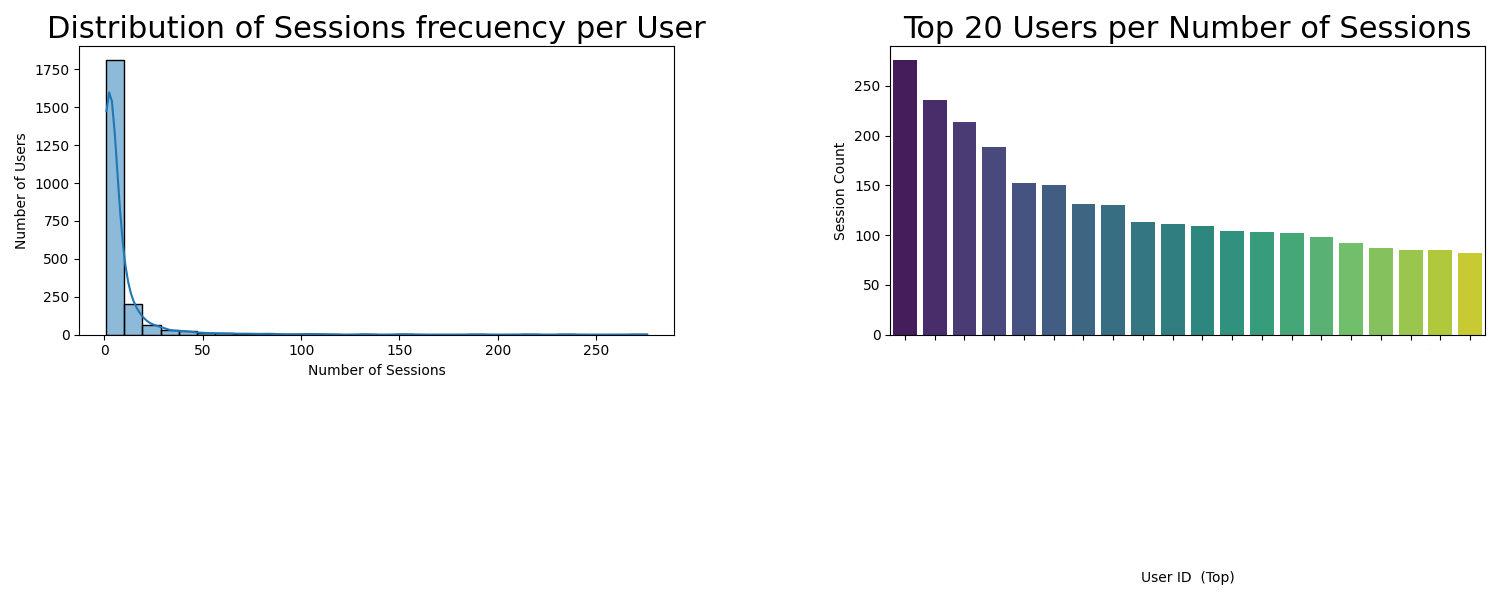
\includegraphics[width=0.8\textwidth]{images/user_dist.png}
    \caption{Distribution of the number of conversations per user (Top 20 most active users).}
    \label{fig:user_dist}
\end{figure}

As shown in Figure \ref{fig:user_dist}, there is a significant variance in user activity. The concentration of data in the most active users allows for a robust analysis of conversational depth, as these long-term interactions are more likely to transition from superficial \textit{cliché} exchanges to more intimate layers of disclosure.


\subsection{Fiability and Quality Standard}
      To validate the reliability of the LLM-based feature extraction (using \textit{Gemma-2-9b-it} as previously mentioned), and provide a benchmark for performance evaluation, a Gold Standard dataset was established. This ground truth consists of 130 carefully selected conversational sessions, manually annotated by human experts to ensure a representative distribution across the different \gls{spt} dimensions and intensity levels.

\subsubsection{Selection Strategy and Sampling Criteria}
The 130 sessions were divided into two primary groups based on their preliminary scoring distributions to ensure that the human evaluators encountered both unambiguous and borderline cases:

\begin{itemize}
    \item \textbf{High-Intensity Group (80 sessions):} This group aimed to capture the most distinct examples of self-disclosure. We selected 20 sessions for each of the three primary categories to which a LLM assigned the maximum intensity score. Additionally, 20 sessions were selected for the non-disclosure baseline, defined as cases where the scores across all categories were strictly lower than 2 ($S_c < 2$).
    
    \item \textbf{Distributional Refinement Group (50 sessions):} This group was curated to test the model's discriminative precision. 
    \begin{itemize}
        \item \textbf{Predominant Category (30 sessions):} 10 sessions per category were chosen under the condition that one specific category had an intensity score $> 3$ and was significantly higher than the scores of the remaining categories.
        \item \textbf{Intermediate Disclosure (20 sessions):} Two subgroups of 10 sessions each were selected based on intermediate scoring ranges to evaluate the model's sensitivity to subtle nuances in the user's narrative.
    \end{itemize}
\end{itemize}

\subsubsection{Human Annotation Protocol}
The labeling process was carried out by a panel of three researchers in the field. To eliminate bias and ensure the integrity of the Gold Standard, the following protocol was implemented:

\begin{enumerate}
    \item \textbf{Blind Evaluation:} Annotators were not provided with the scores previously generated by the reference LLM  model.
    \item \textbf{Scoring Metric:} Each session was manually evaluated by every annotator using a standardized scale from 0 to 5, matching the rubric used in the categories prompt (See Appendix \ref{appendix:prompt_categories}).
    \item \textbf{Independent Review:} Evaluators worked independently to assess the presence and intensity of disclosure in each of the three theoretical categories.
\end{enumerate}

This curated dataset serves as the definitive reference for calculating the error margins, providing a statistically sound foundation for the subsequent analysis of results. 


\subsubsection{Validation of the gold standard: Interagreement}

To assess the reliability of the human-annotated benchmark, we calculated the Cohen's Kappa coefficient across all pairs of evaluators for the three primary categories. The results, illustrated in Figure \ref{fig:interagreement}, show agreement levels ranging from 0.32 to 0.52, which conventionally corresponds to "fair" to "moderate" agreement.

While these values may appear numerically low, they are expected and justified within the context of natural language processing for sensitive populations for the following reasons:

\begin{itemize}
    \item \textbf{Subjectivity of Intimacy:} Interpreting "depth" in elderly self-disclosure is inherently non-binary; a score of 3 versus 4 often depends on individual evaluator perception of vulnerability.
    \item \textbf{Thematic Overlap:} SPT categories are fluid; complex disclosures (e.g., family loss) frequently trigger multiple categories ($C_2$ and $C_3$), fragmenting agreement.
    \item \textbf{Metric Sensitivity:} Cohen's Kappa penalizes any 1-point difference on a 6-level scale (0-5) as a total disagreement, even when annotators agree on the general presence and intensity of a topic.
\end{itemize}
%This inherent human variance underscores the difficulty of the task and establishes the necessity for the \textbf{Methodological Axes} defined in this study. By identifying these discrepancies, we can demonstrate that the LLM-based extraction—specifically the gating mechanism in Experiment A—serves as a tool for \textbf{inferential stabilization}, providing a consistent "algorithmic consensus" that human intuition alone cannot maintain at scale.

\begin{figure}[htbp]
    \centering
    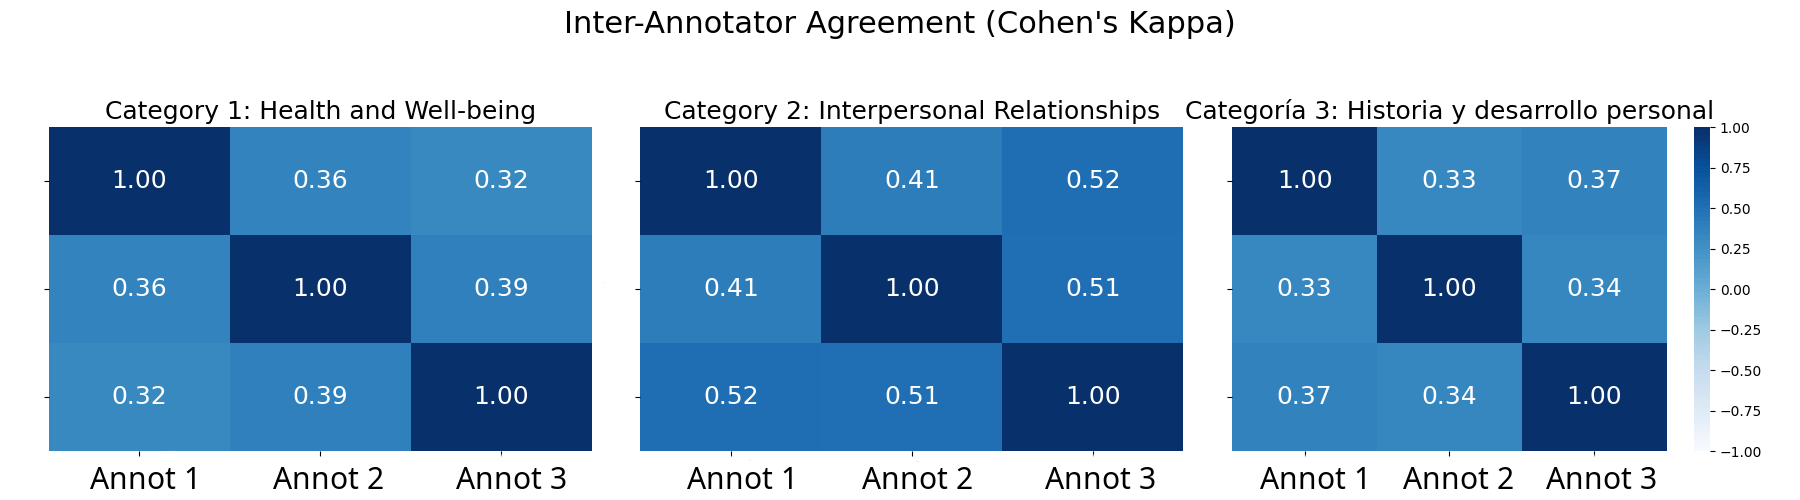
\includegraphics[width=\textwidth]{images/interagreement.png}
    \caption{Inter-Annotator Agreement (Cohen's Kappa) across the three primary categories.}
    \label{fig:interagreement}
\end{figure}
%\newpage

%While Cohen's Kappa captures exact categorical matches, it can be overly conservative for ordinal data. 
Therefore, we applied Krippendorff’s Alpha ($\alpha$), Mean Point Distance, and Spearman Correlation ($\rho$) to assess the "distance" between human ratings. Table \ref{tab:reliability_metrics} summarizes the consistency across the three primary categories.

\begin{table}[htbp]
\centering
\caption{Consolidated Reliability Metrics for the Gold Standard Dataset.}
\label{tab:reliability_metrics}
\begin{tabular}{@{}lccc@{}}
\toprule
\textbf{Category} & \textbf{Krippendorff's $\alpha$} & \textbf{Avg. Point Distance} & \textbf{Mean Spearman $\rho$} \\ \midrule
$C_1$: Health and Well-being & 0.6634 & 0.96 & 0.70 \\
$C_2$: Interpersonal Relationships & 0.8311 & 0.66 & 0.83 \\
$C_3$: Personal History & 0.6698 & 0.80 & 0.69 \\ \bottomrule
\end{tabular}
\end{table}

The analysis reveals several insights into the quality of the human-labeled benchmark:

\begin{itemize}
    \item \textbf{High Consistency in $C_2$:} Interpersonal Relationships achieved the highest reliability ($\alpha = 0.83$), suggesting that experts find social dynamics easier to quantify than health or historical nuances.
    \item \textbf{Sub-Point Error Margin:} Across all categories, the average discrepancy between any two evaluators is consistently below 1.0 points on the 0-5 scale. This indicates that even when annotators disagree, they remain within a close numerical range, validating the stability of the intensity rubric.
    \item \textbf{Strong Linear Trends:} The high Spearman Correlation values (averaging $\sim$0.74) confirm that evaluators identify the same relative peaks and valleys of self-disclosure, even if their absolute baseline scores vary slightly.
\end{itemize}

In conclusion, these results confirm that the Gold Standard is a robust reference. The low average distance ($< 1.0$) suggests that the experimental results (Exp. A, B, and C) can be evaluated with a high degree of confidence, as the ground truth provided by humans is mathematically consistent despite its inherent subjectivity.



\subsection{Evaluation of the Metodological Axes}


\subsubsection{Impact of Prompt Architecture on Extraction Accuracy}

A comparative analysis of the prompt engineering strategies reveals that consolidated inference outperforms fragmented requests (See Table \ref{tab:experiment_names_updated}: Architecture). As illustrated in Figure \ref{fig:error_distribution}, the single-prompt approach exhibits a highly favorable error distribution, with a significant concentration of errors at the 0 and 1 levels. In contrast, the multi-prompt architecture flattens this curve, showing a concerning increase in higher-magnitude errors (3 to 5 range), suggesting that isolating categories may lead to ``intensity drift" or over-sensitization by the LLM.


\begin{figure}[htbp]
    \centering
    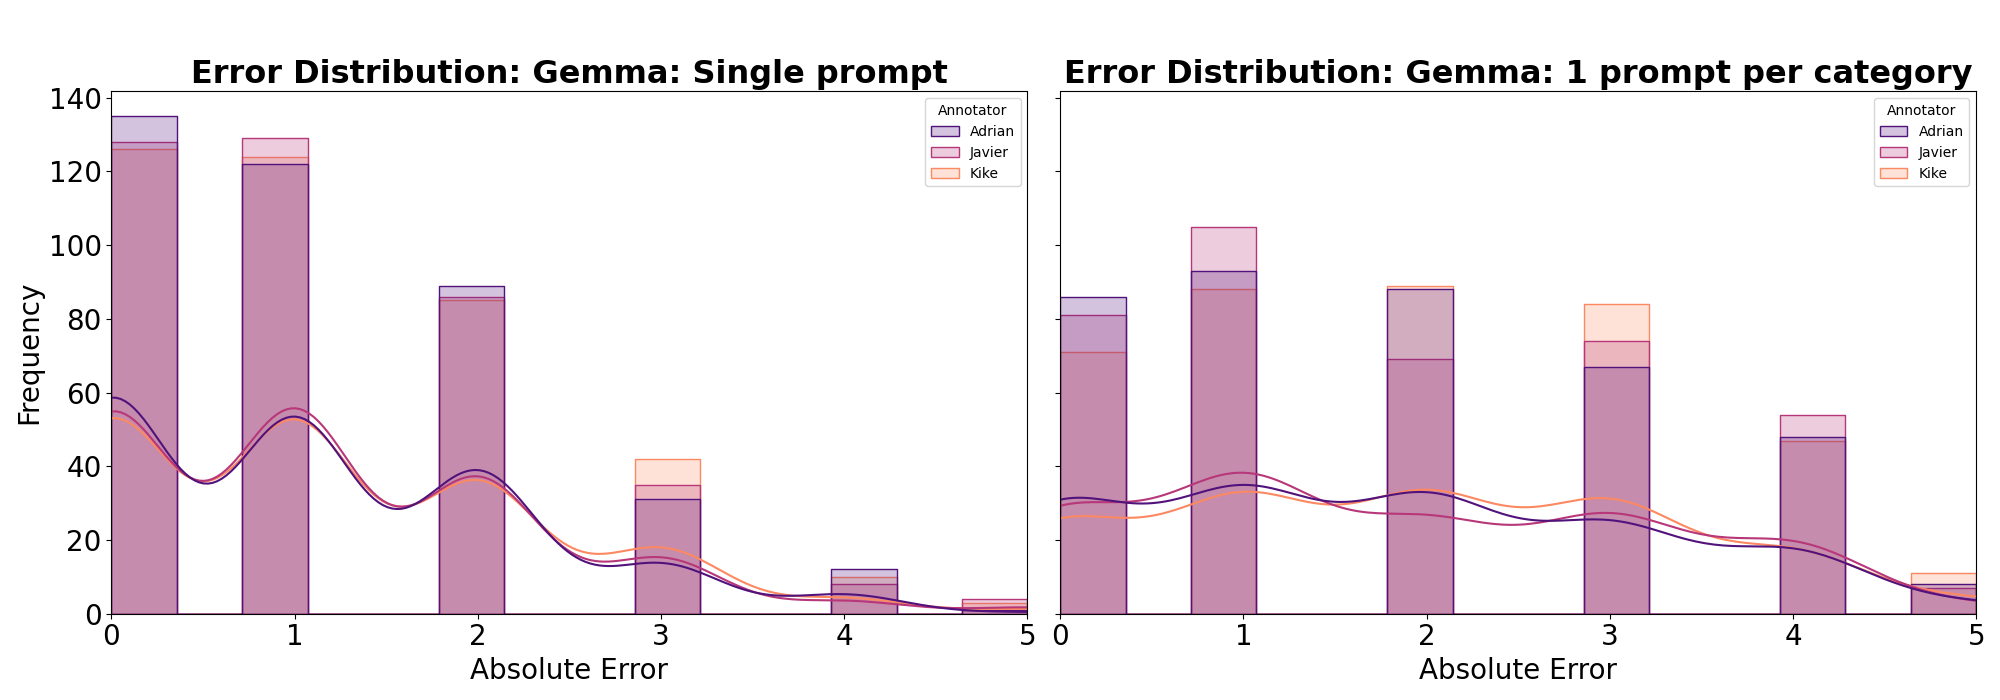
\includegraphics[width=0.9\textwidth]{images/1vs3MAE.png}
    \caption{Error dispersion comparison: single prompt vs one prompt per category.}
    \label{fig:error_distribution}
\end{figure}


This trend is quantitatively validated by the Mean Absolute Error (MAE) benchmarks shown in Figure \ref{fig:mae_combined}. The data reveals two key insights:

\begin{itemize}
    \item \textbf{Categorical Consistency (Figure \ref{fig:mae_category}):} The single-prompt model achieves a lower MAE across all three theoretical dimensions. Notably, in the \textit{Interpersonal Relationships} category, the error drops below 1.0, whereas the multi-prompt setup consistently remains above the 1.5 threshold.
    \item \textbf{Annotator Alignment (Figure \ref{fig:mae_annotator}):} The single-prompt architecture maintains a stable error margin ($\approx 1.2$) regardless of the human evaluator, whereas the multi-prompt approach introduces higher variance and significantly higher average error ($\approx 1.8$ to $1.9$).
\end{itemize}

The success of the single-prompt strategy likely stems from contextual coherence. By evaluating all dimensions within a single context window, the model can maintain a relative scale of intensity across categories, preventing the hallucination that occurs when the LLM is forced to find a score for a specific topic in isolation.

\begin{figure}[htbp]
    \centering
    
    \begin{subfigure}[b]{0.49\textwidth}
        \centering
        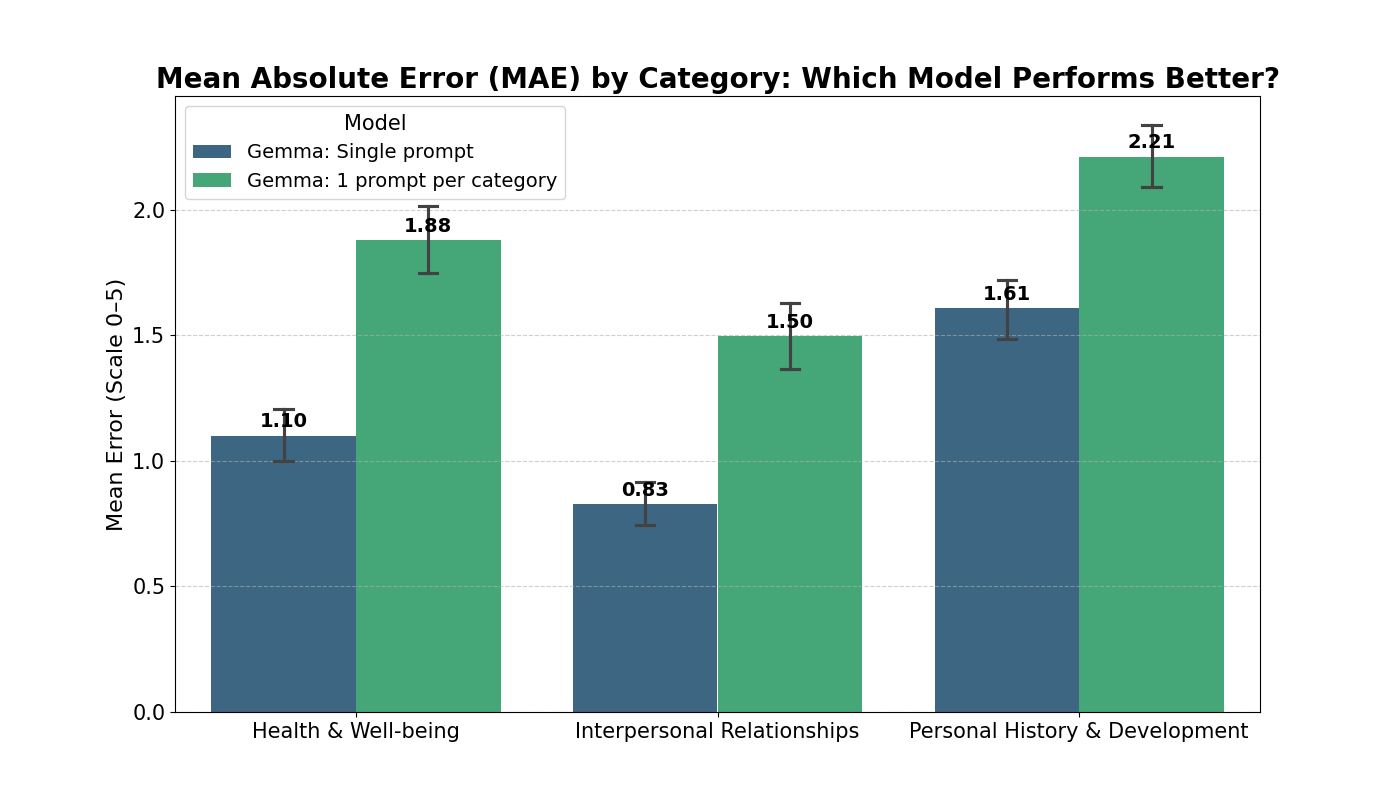
\includegraphics[width=\textwidth]{images/de1vs3peticiones.png}
        \caption{MAE by category}
        \label{fig:mae_category}
    \end{subfigure}
    \hfill
    \begin{subfigure}[b]{0.49\textwidth}
        \centering
        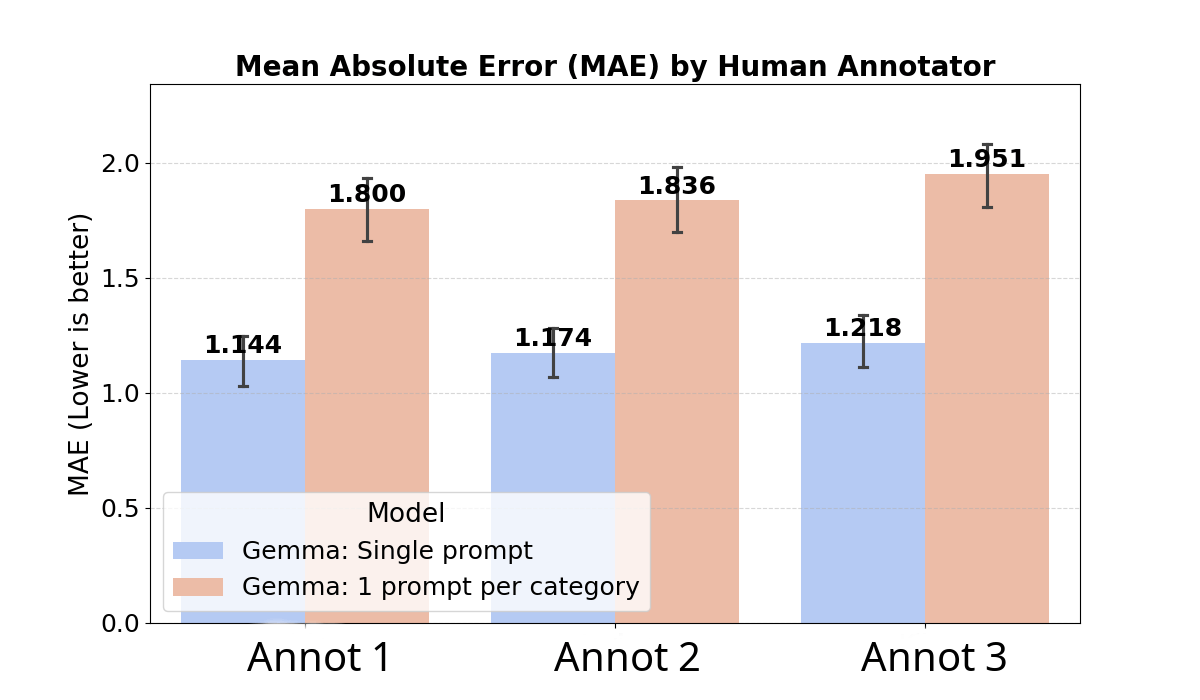
\includegraphics[width=\textwidth]{images/MAE_por_evaluador.png}
        \caption{MAE by annotator}
        \label{fig:mae_annotator}
    \end{subfigure}
    
    \caption{Comparison of Mean Absolute Error (MAE) across categories and annotators.}
    \label{fig:mae_combined}
\end{figure}

\subsubsection{Impact of Scale Granularity on Normalized Error}

To evaluate the precision of the LLM against the human Gold Standard, we normalized the error across three experimental configurations: Exp\_5 (0--5 scale), Exp\_3 (0--3 scale), and Exp\_2 (binary/simplified). The results indicate that scale complexity is a primary driver of inferential variance. (See Table \ref{tab:experiment_names_updated}: Granularity)

\begin{itemize}
    \item \textbf{Optimal Performance in Simplified Scales:} As shown in the heatmap (Figure \ref{fig:heatmap_normalized_error}), the Exp\_2 configuration achieves the lowest Global Mean Error (0.216). This suggests that while high-granularity scales (0--5) capture more nuance, they do not significantly introduce   more noise into the LLM's decision-making process.
 
\begin{figure}[htbp]
    \centering
    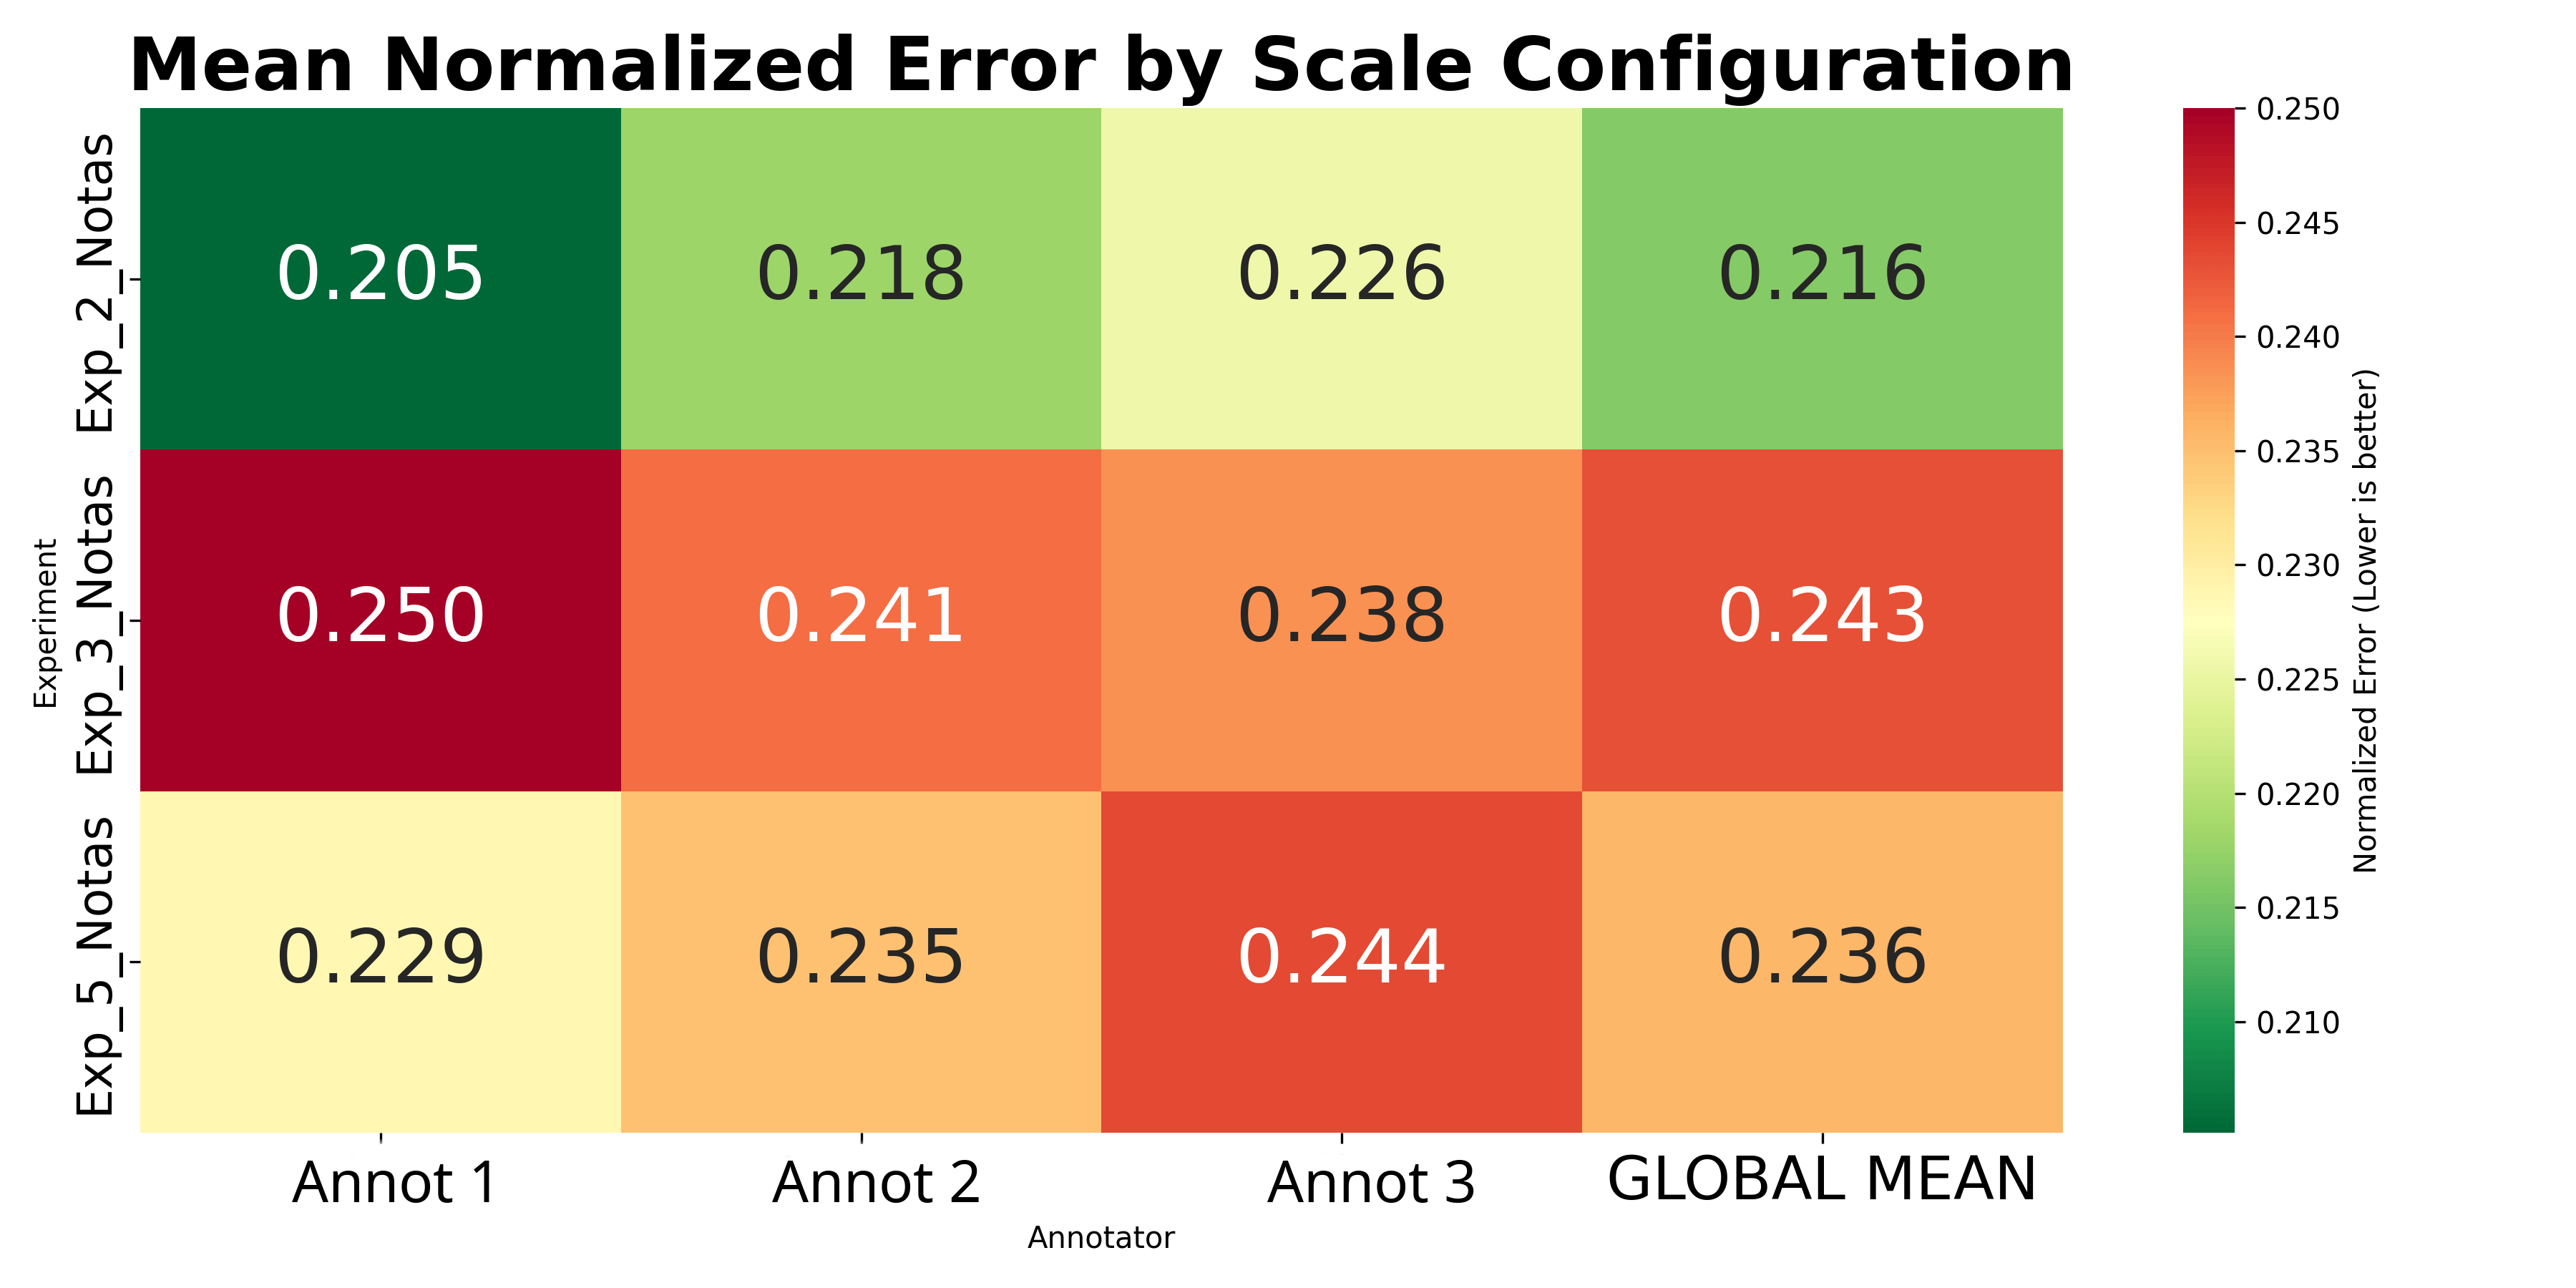
\includegraphics[width=0.7\textwidth]{images/mean_normalized_error.png}
    \caption{Mean normalized error (0--1) by experiment and annotator. Lower values indicate better performance.}
    \label{fig:heatmap_normalized_error}
\end{figure}

    \item \textbf{Error Stability across Categories:} Figure \ref{fig:boxplots_category} illustrates that while error is generally suppressed in Exp\_2, the \textit{Personal History} category exhibits a higher error ceiling. This indicates that complex, narrative-heavy disclosures are less amenable to drastic scale reduction compared to more objective topics like health.

    
\begin{figure}[htbp]
    \centering
    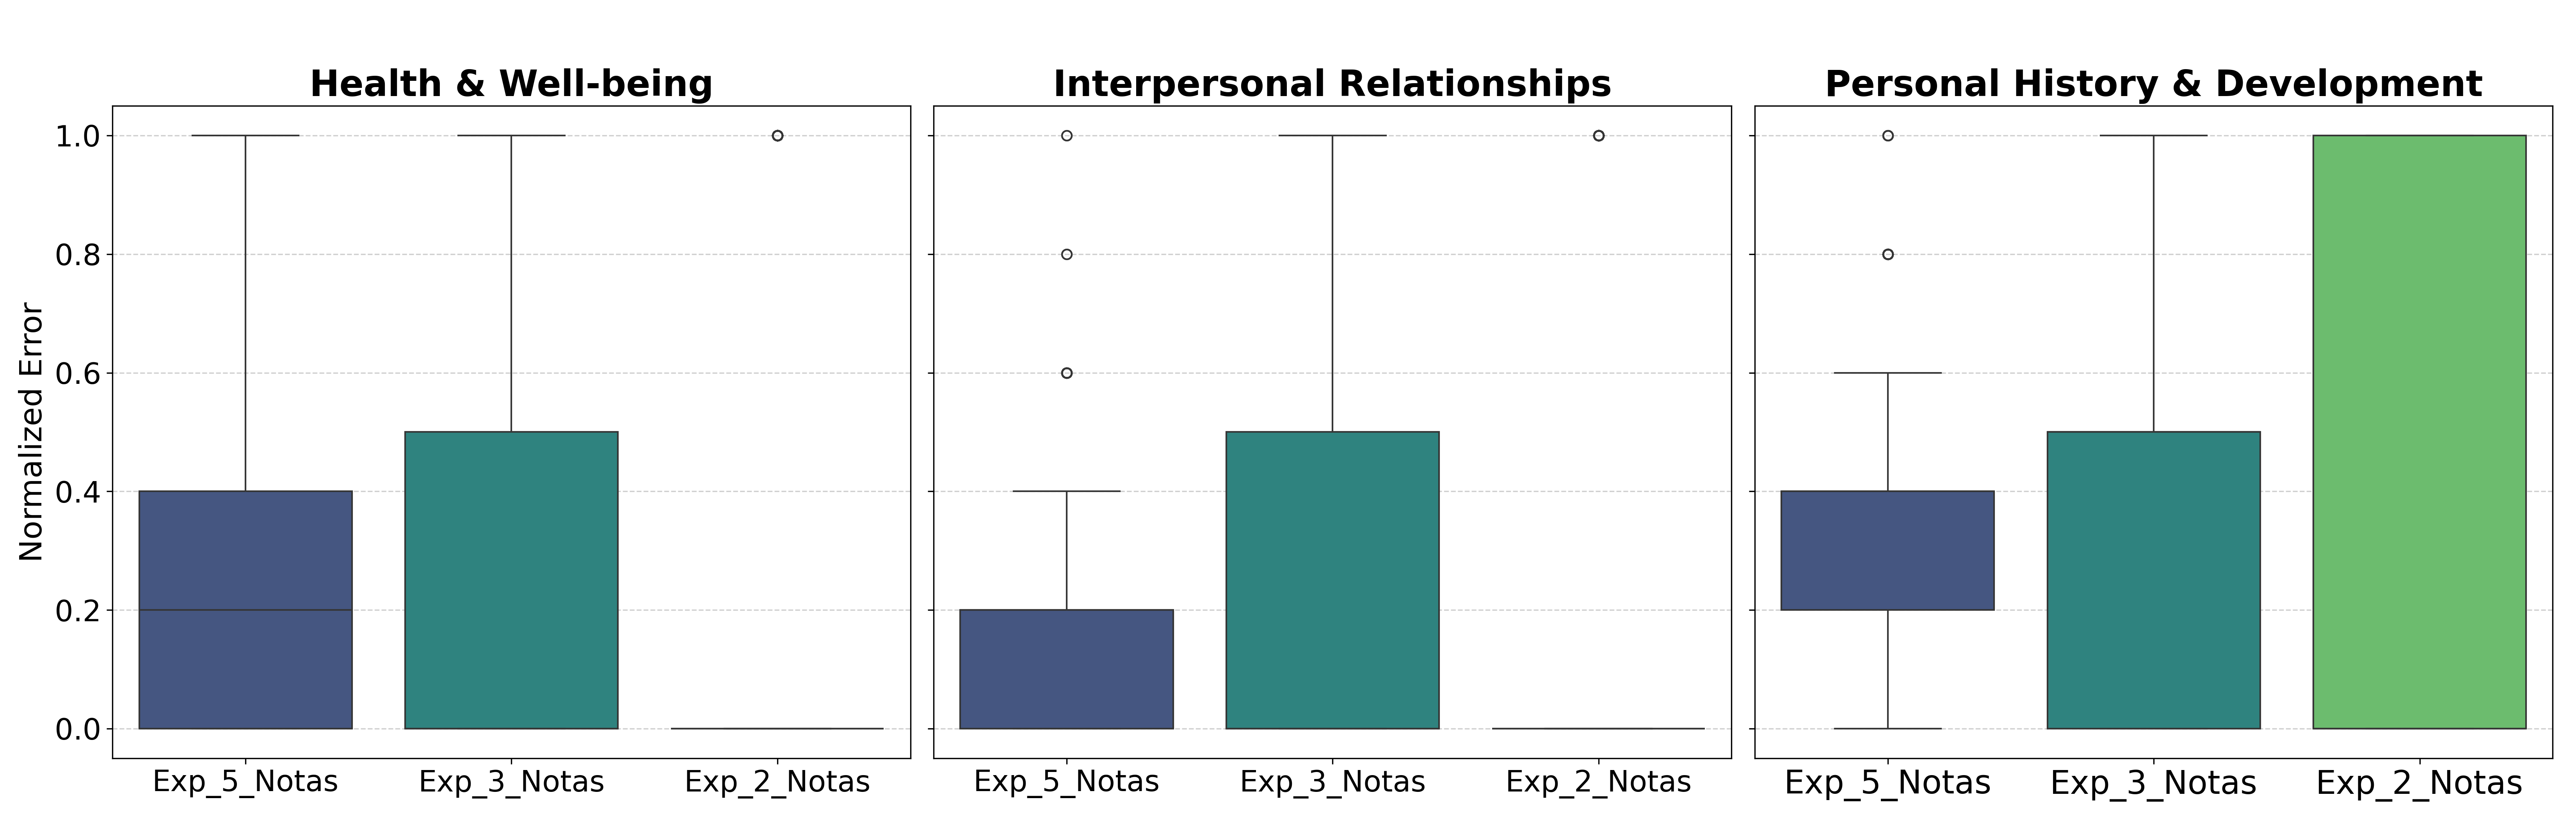
\includegraphics[width=0.95\textwidth]{images/comparative_scales_boxplots.png}
    \caption{Normalized error distribution by category across different scale configurations.}
    \label{fig:boxplots_category}
\end{figure}



    \item \textbf{Annotator Invariance:} The consistent error distribution across the three annotators in Figure \ref{fig:boxplots_evaluator} confirms that the model's performance is not biased toward any specific human evaluator's style. The LLM maintains a systematic error profile, which is crucial for large-scale data processing where human consistency naturally fluctuates.

    

\begin{figure}[htbp]
    \centering
    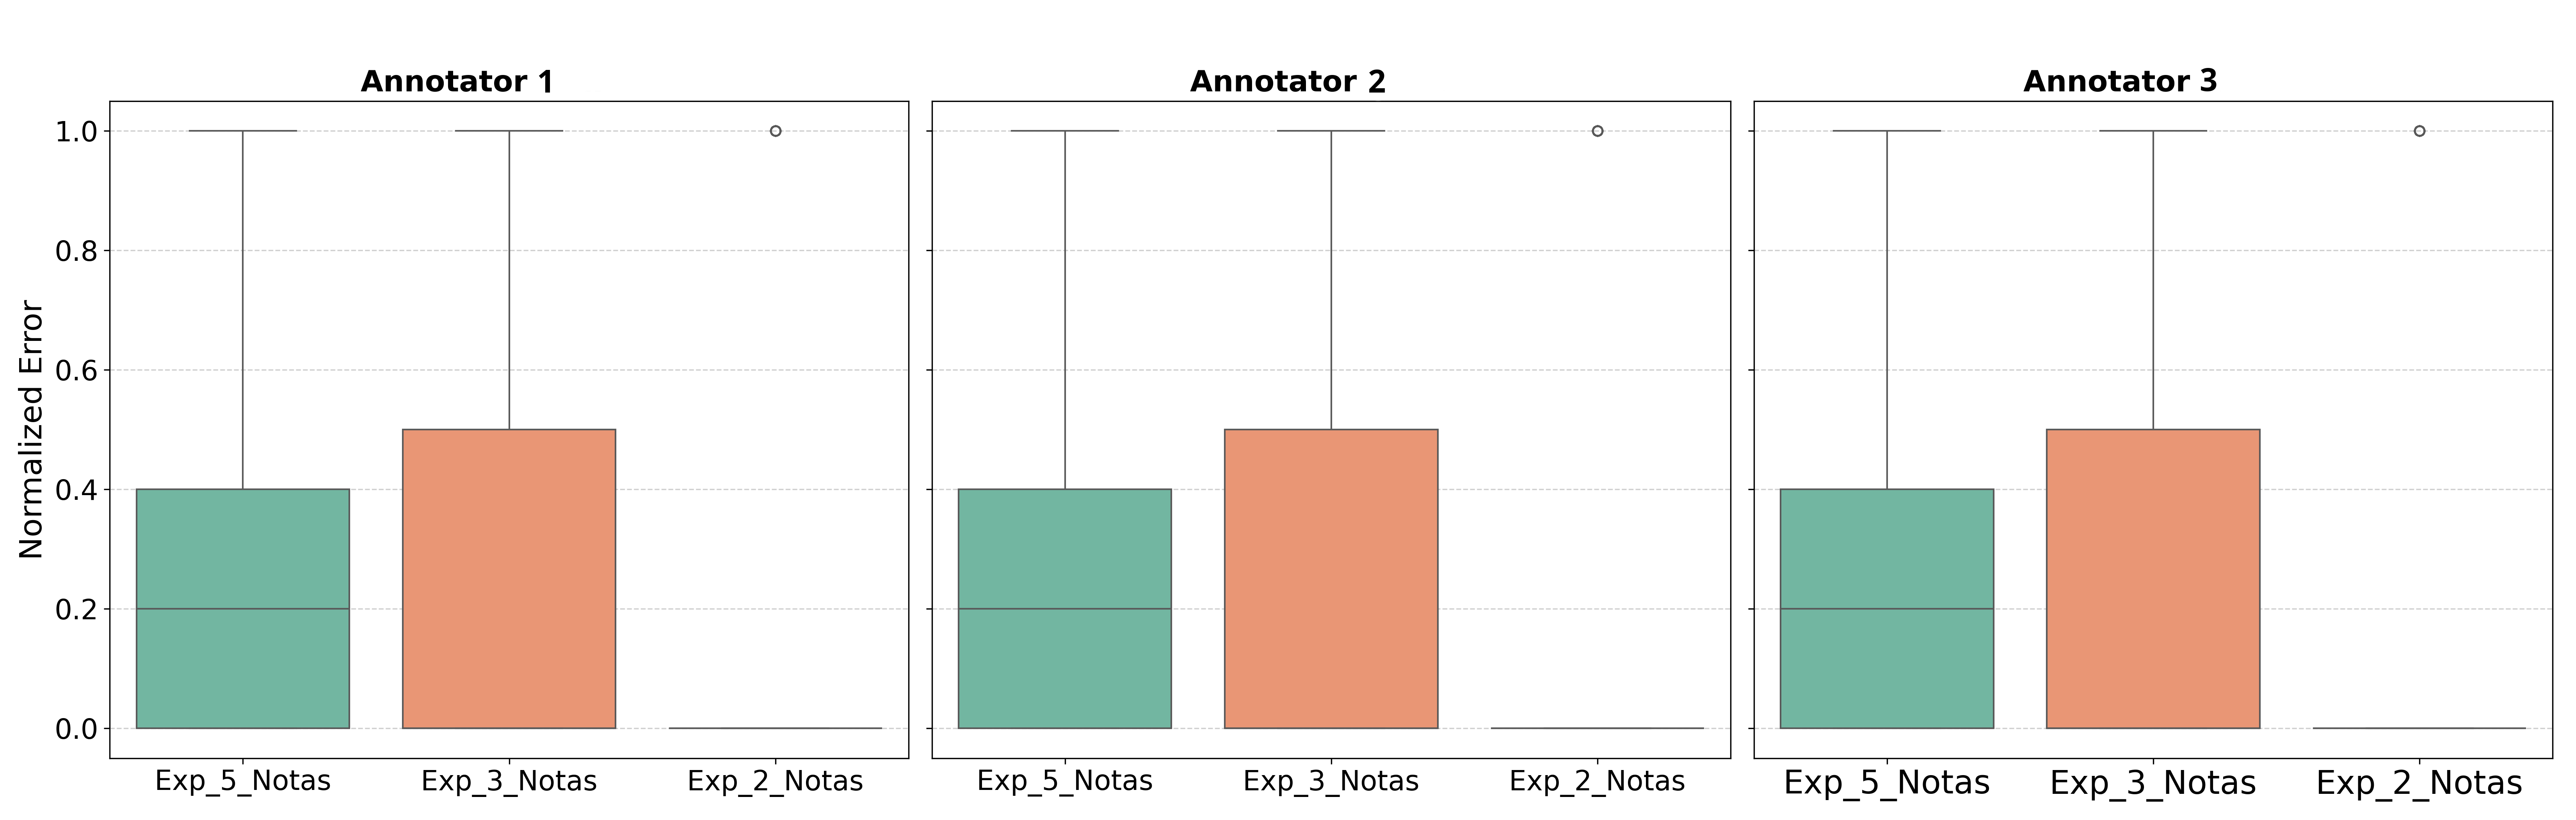
\includegraphics[width=0.95\textwidth]{images/comparative_scales_boxplots_anot.png}
    \caption{Normalized error distribution by anotator across different scale configurations .}
    \label{fig:boxplots_evaluator}
\end{figure}

\end{itemize}

Ultimately, these findings justify the use of Exp\_5 for qualitative depth, but also highlight that for tasks requiring high statistical reliability, a reduction in scale granularity (toward the Exp\_2 model) significantly stabilizes the output.



\newpage
\subsubsection{Comparative Analysis of Fusion and Aggregation Strategies}

The results from the final experimental axis (See Table \ref{tab:experiment_names_updated}: Granularity), synthesized in figures \ref{fig:normalized_error_heatmap} and \ref{fig:absolute_error_grid}, confirm that the mathematical method used to combine sub-topic scores is as critical as the prompt structure itself. 

\begin{itemize}
    \item \textbf{Superiority of the Gating Mechanism (Hadamard):} The data reveals that the \gls{hadamard} product architecture consistently yields the lowest error margins. As seen in Figure \ref{fig:normalized_error_heatmap}, the ``Had" experiments (Exp2, Exp5, and Exp8) outperform the ``Mean" and ``Max" counterparts across every scale (Formula \ref{eq:hadamard}). Specifically, Exp2\_Bin\_Had achieves the lowest global normalized error (0.196), proving that binary gating effectively filters out hallucinated intensity by requiring explicit topic confirmation.
    \item \textbf{Distribution and Tail Stability:} Figure \ref{fig:absolute_error_grid} provides a granular view of this stability. In the ``Had" rows, the absolute error distributions show a higher concentration at the zero-error mark and a significantly ``thinner" tail compared to ``Mean" models. This suggests that Mean fusion tends to ``dilute" significant disclosures, while Hadamard gating ensures that intensity is only recorded when the semantic presence is strictly validated.
    \item \textbf{The Depth-Reliability Trade-off:} While Exp2 (Binary) is technically the most precise, Exp8\_5R\_Had maintains a nearly identical error profile (0.199) while providing a 0--5 granularity. This justifies the selection of the 5-level rubric combined with Hadamard gating as the optimal architecture for capturing conversational depth.
\end{itemize}

Ultimately, these findings indicate that a gated architecture acts as a robust semantic filter, bridging the gap between high-granularity qualitative data and quantitative statistical reliability.
\begin{figure}[!htbp]
    \centering
    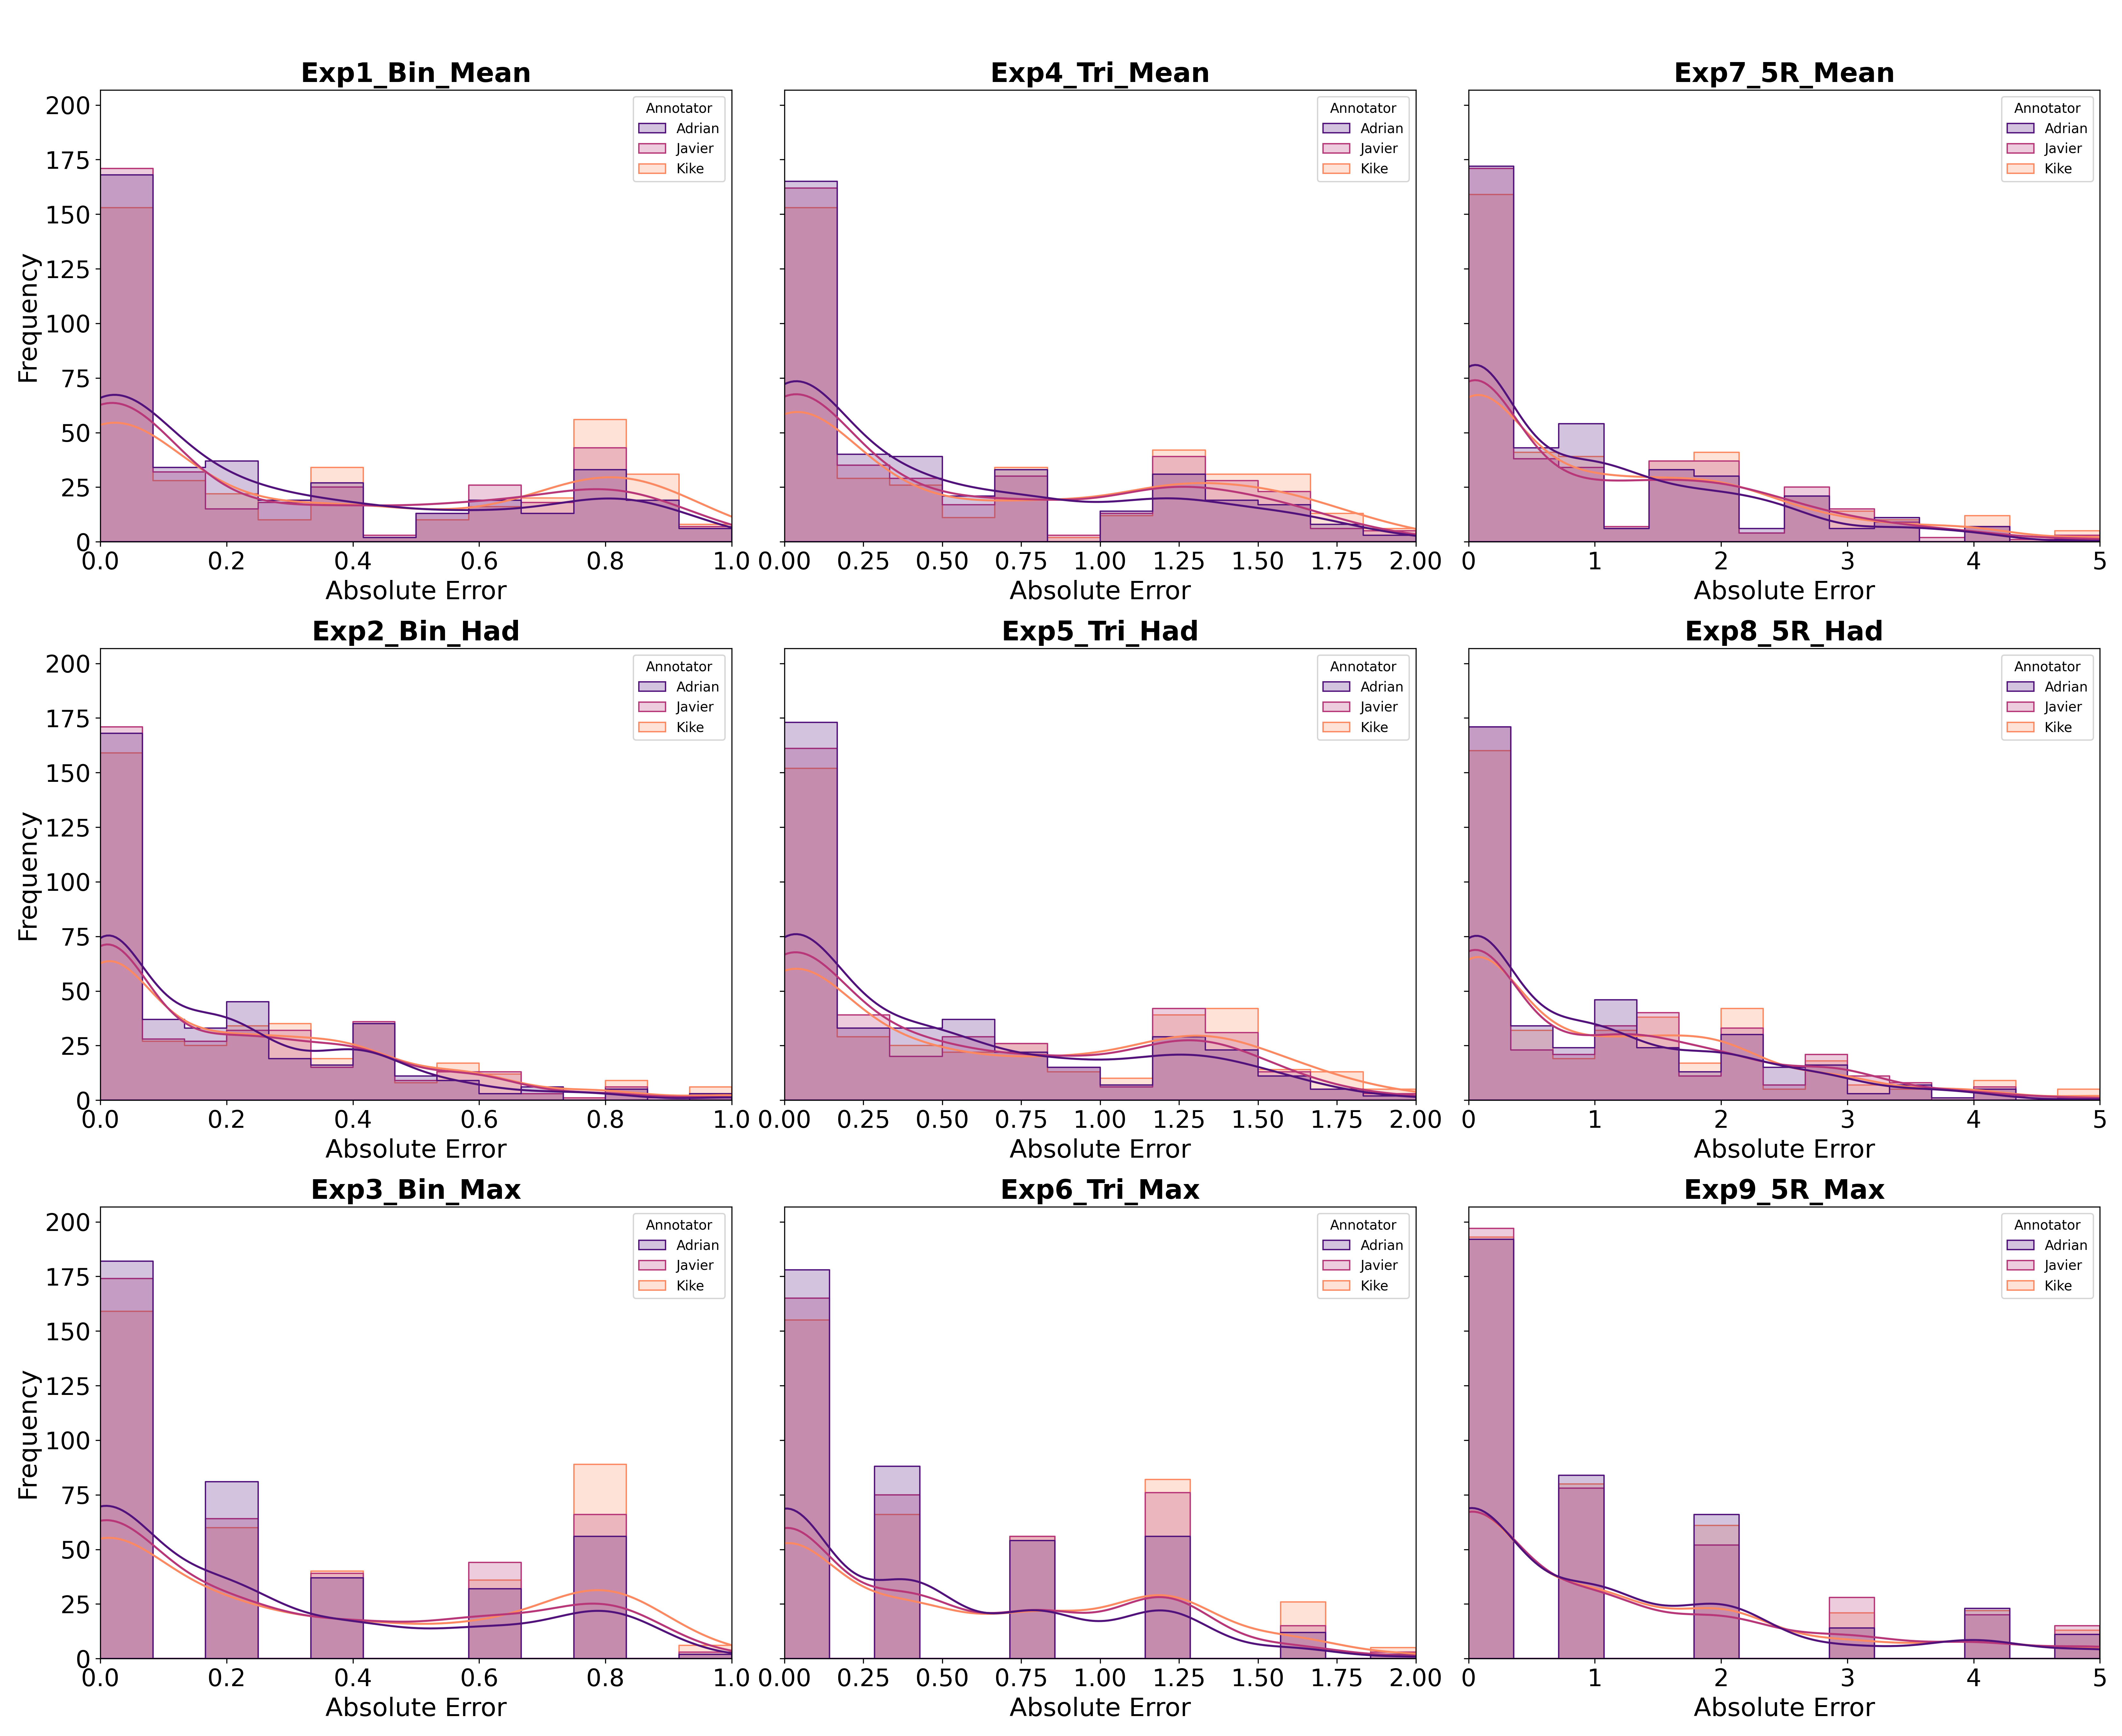
\includegraphics[width=0.95\textwidth]{images/absolute_error_grid.png}
    \caption{Absolute error distributions across all scale configurations and annotators (3×3 layout).}
    \label{fig:absolute_error_grid}
\end{figure}

\begin{figure}[!htbp]
    \centering
    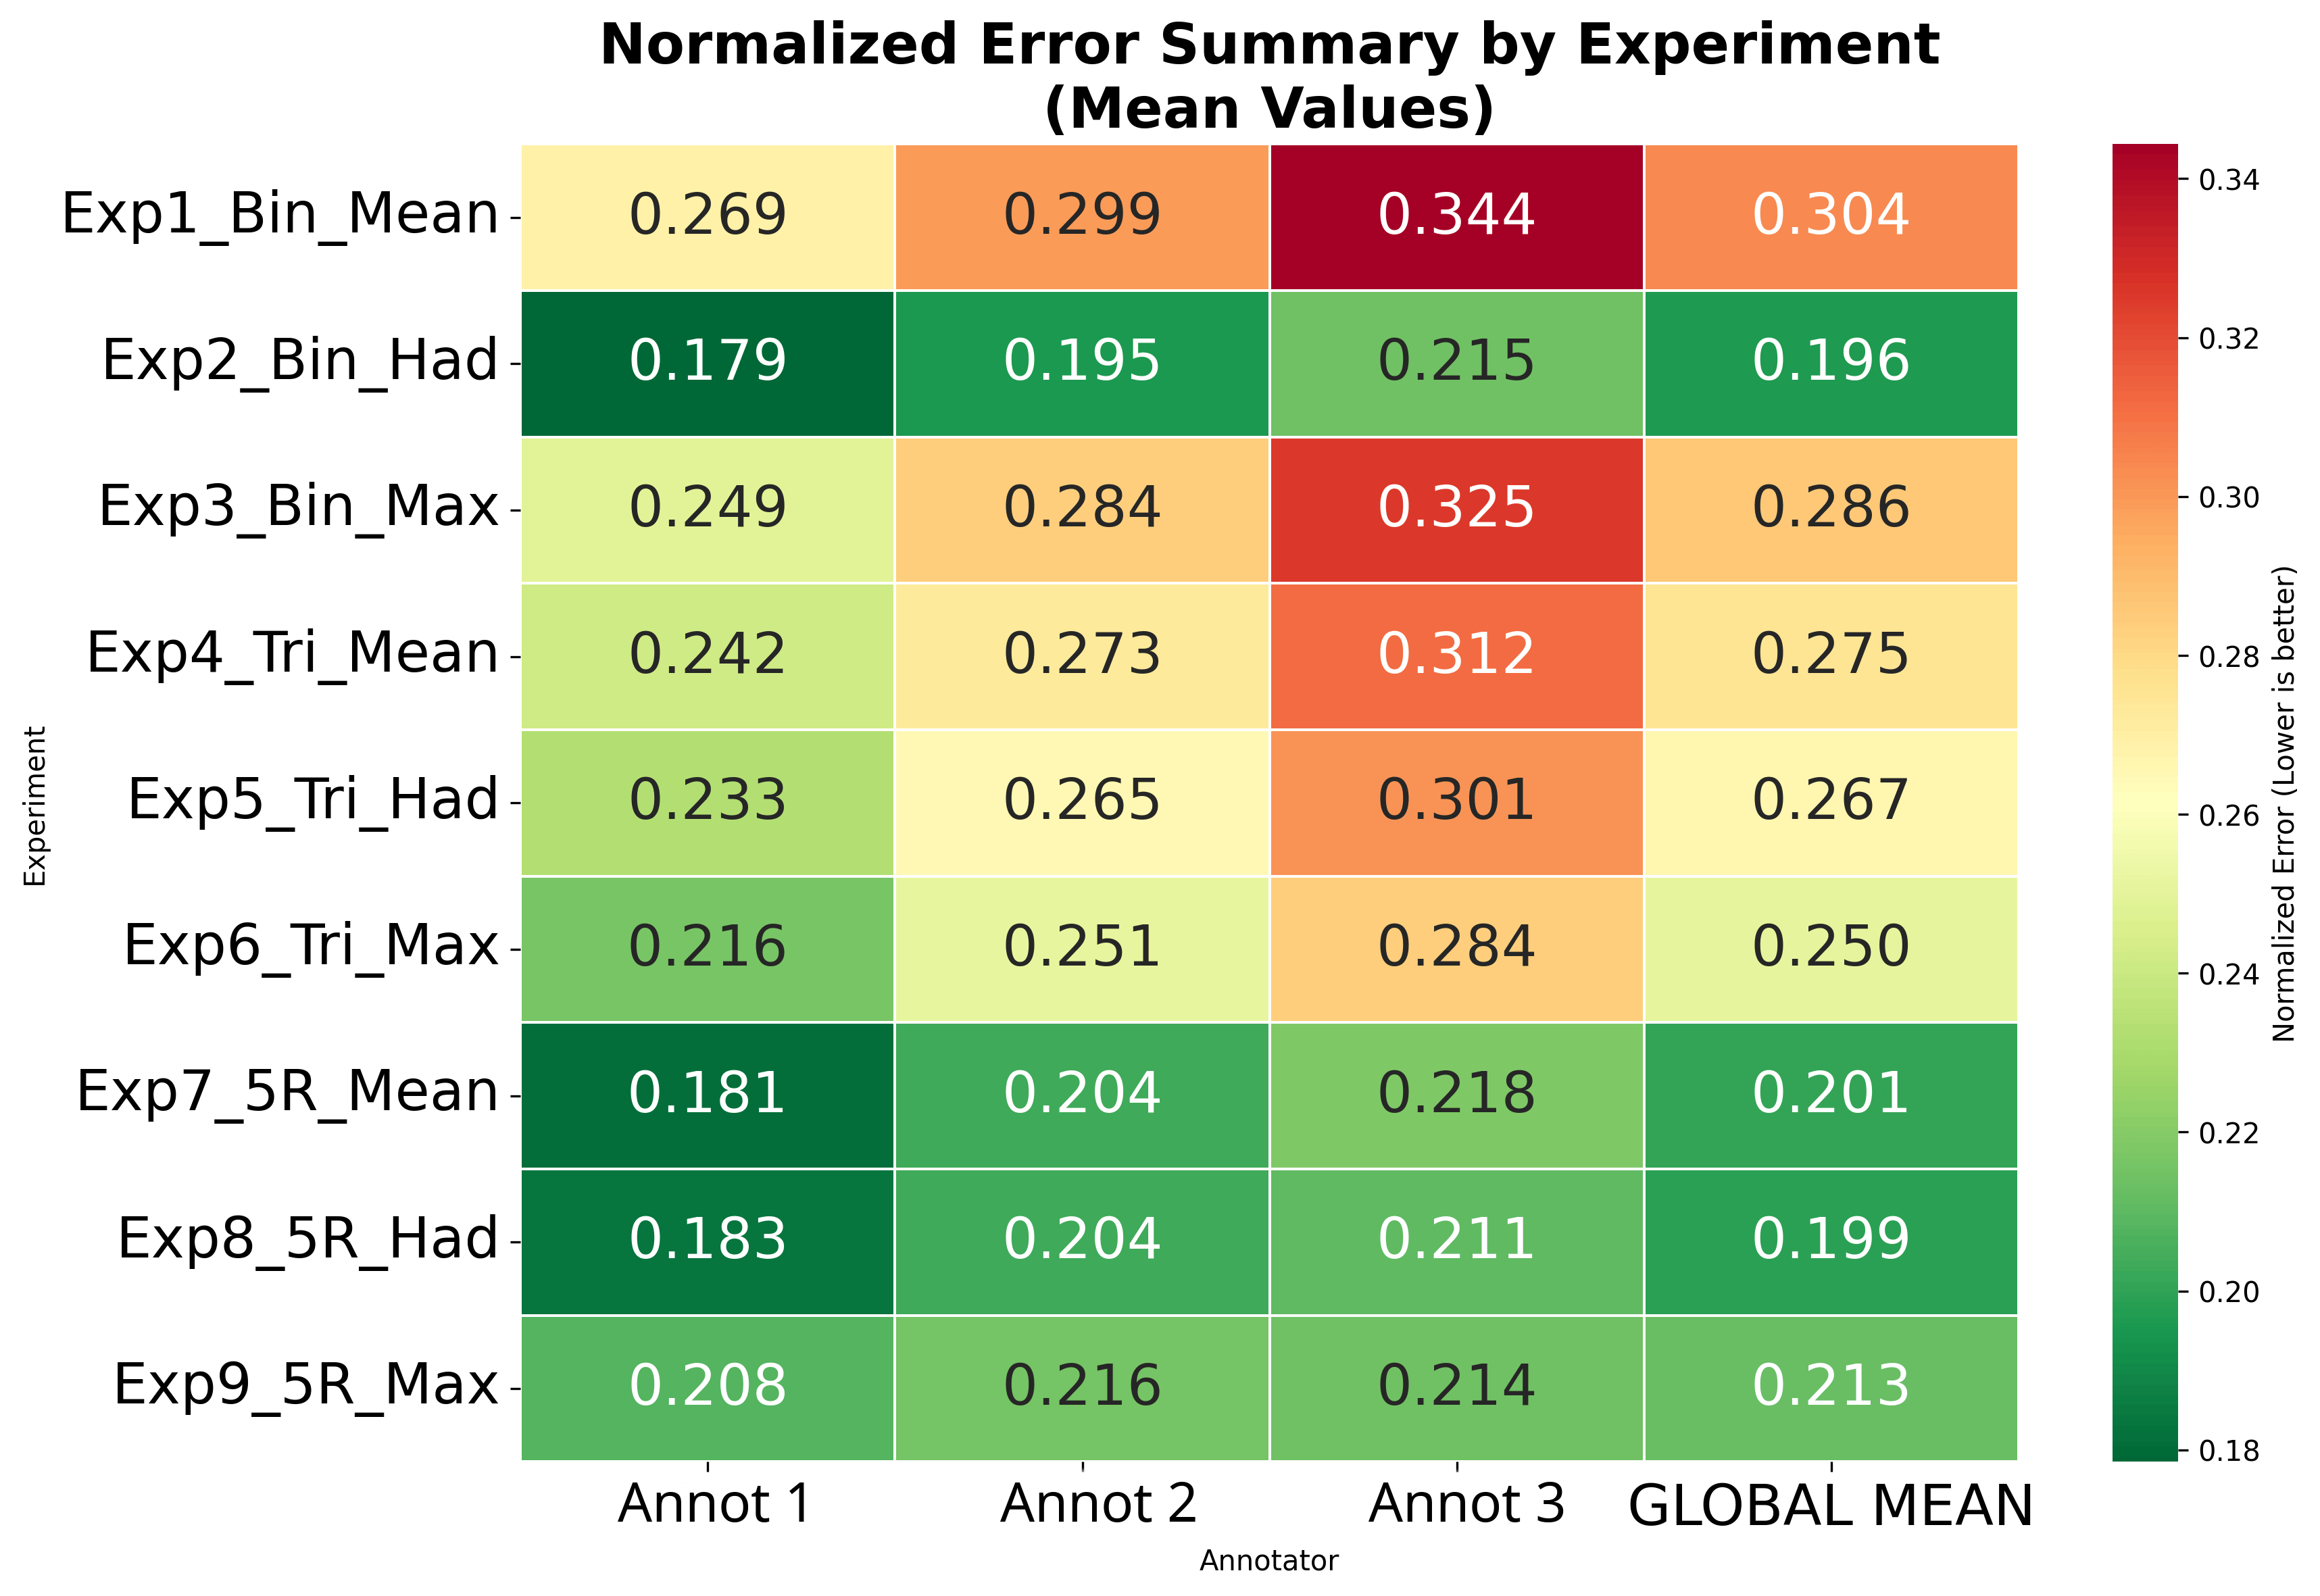
\includegraphics[width=0.75\textwidth]{images/normalized_error_heatmap.png}
    \caption{Mean normalized error by experiment and annotator. Lower values indicate better performance .}
    \label{fig:normalized_error_heatmap}
\end{figure}



\newpage
\subsection{Centroid Definition and Cluster Population Dynamics}

The analysis of the clustering results across the different experimental setups (those in Table \ref{tab:experiment_names}) reveals a consistent inverse relationship between centroid definition and cluster size. As observed in Figures \ref{fig:binary_hadamard}, \ref{fig:subtopic_rubric}, and \ref{fig:subtopic_binary}, the clusters characterized by highly defined centroids, representing high-intensity, specific self-disclosure, tend to have smaller populations. This suggests that while intense, thematic disclosure exists, it is a particular behavior within the elderly-chatbot interaction space.


This dynamic is further evidenced by the following patterns:
\begin{itemize}
    \item \textbf{Residual Absorption:} Sessions that do not exhibit a clear thematic focus or high intensity are naturally sequestered into the residual cluster ($+1$ cluster). This group acts as a semantic sink for interactions that are either superficial (cliché-level) or highly fragmented, preventing them from diluting the purity of the three primary archetypes.
    %\item \textbf{Impact of Methodological Axes:} This phenomenon is particularly pronounced in the experiments that utilized the superior research axes \textcolor{red}{esto no está claro, refiérelo de otra forma}, such as the \textbf{Hadamard gating mechanism} (see Figure \ref{fig:binary_hadamard}). By effectively filtering noise and "hallucinated" intensities, these refined axes produce sharper, more isolated centroids. Consequently, the boundary between "thematically pure" sessions and "residual noise" becomes significantly clearer.
    \item \textbf{Resolution vs. Fragmentation:} In contrast, less robust configurations (Figure \ref{fig:rubric_based_hadamard}, \ref{fig:topic_rubric} and \ref{fig:topic_binary}) result in more diffuse, less defined clusters. In those cases, the lack of a strong gating signal causes ambiguous sessions to bleed into the primary categories, reducing the qualitative interpretability of the results.
\end{itemize}

Ultimately, these results validate the $3+1$ architecture. The concentration of noise into a single, non-specific cluster allows for a much more precise characterization of the three core behavioral profiles, proving that the methodological refinements introduced in the extraction phase are essential for identifying true patterns of social penetration.

% 1: Rubric Based Hadamard Fusion
\begin{figure}[htbp]
    \centering
    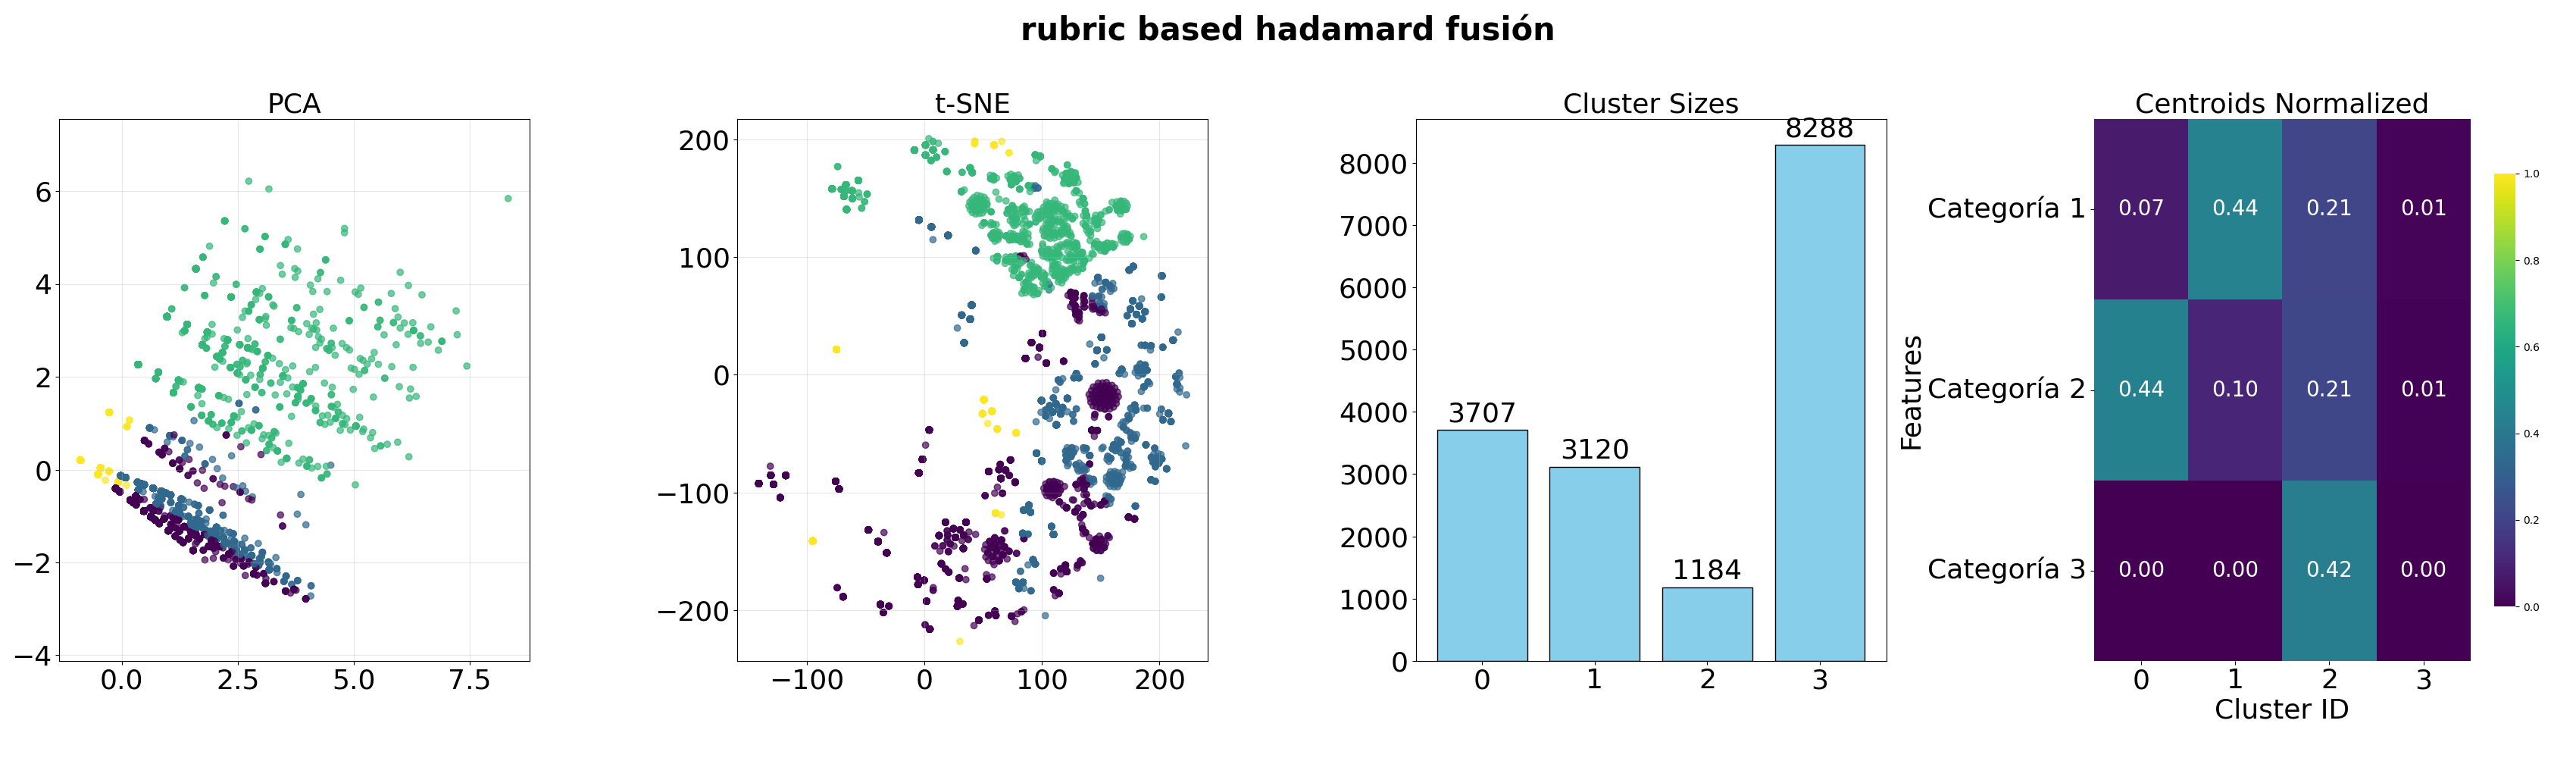
\includegraphics[width=\textwidth]{images/rubric_based_hadamard_fusión.png}
    \caption{Rubric Based Hadamard Fusion experiment.}
    \label{fig:rubric_based_hadamard}
\end{figure}

% 2: Binary Hadamard Fusion
\begin{figure}[htbp]
    \centering
    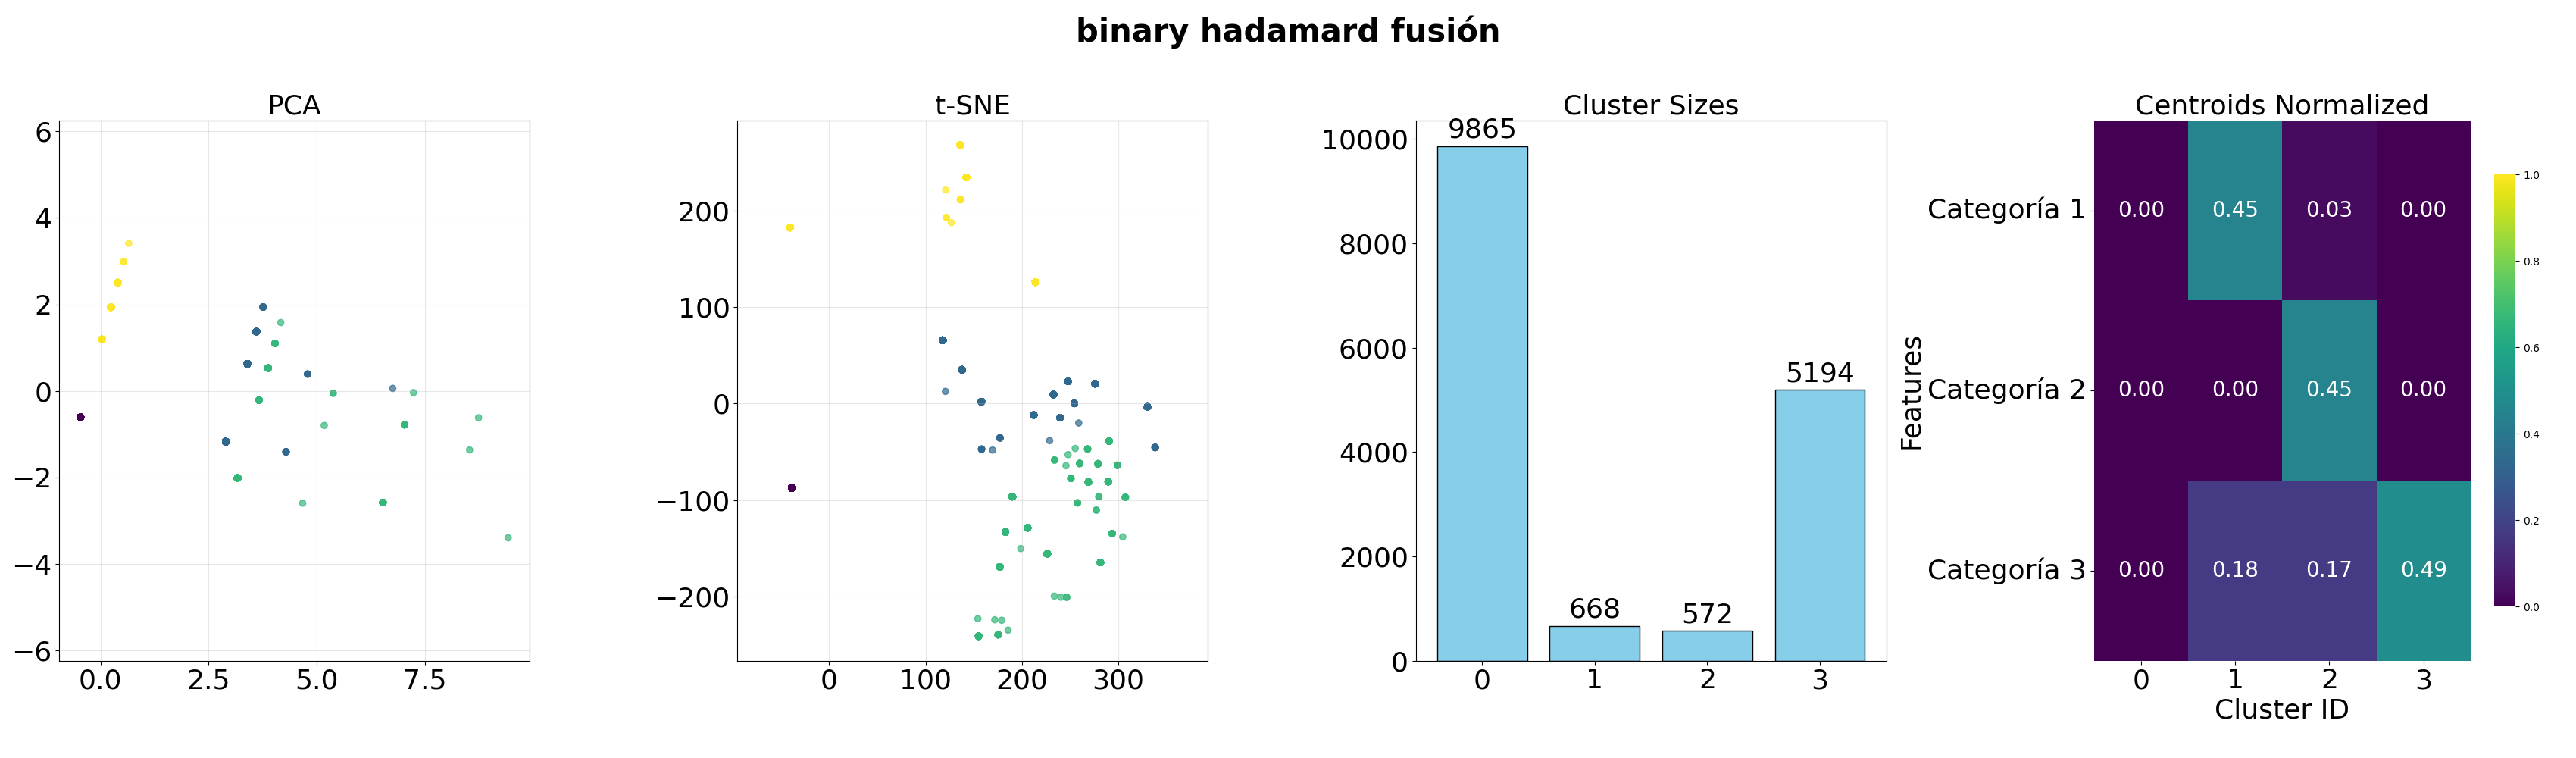
\includegraphics[width=\textwidth]{images/binary_hadamard_fusión.png}
    \caption{Binary Hadamard Fusion experiment.}
    \label{fig:binary_hadamard}
\end{figure}

% 3: Topic Rubric
\begin{figure}[htbp]
    \centering
    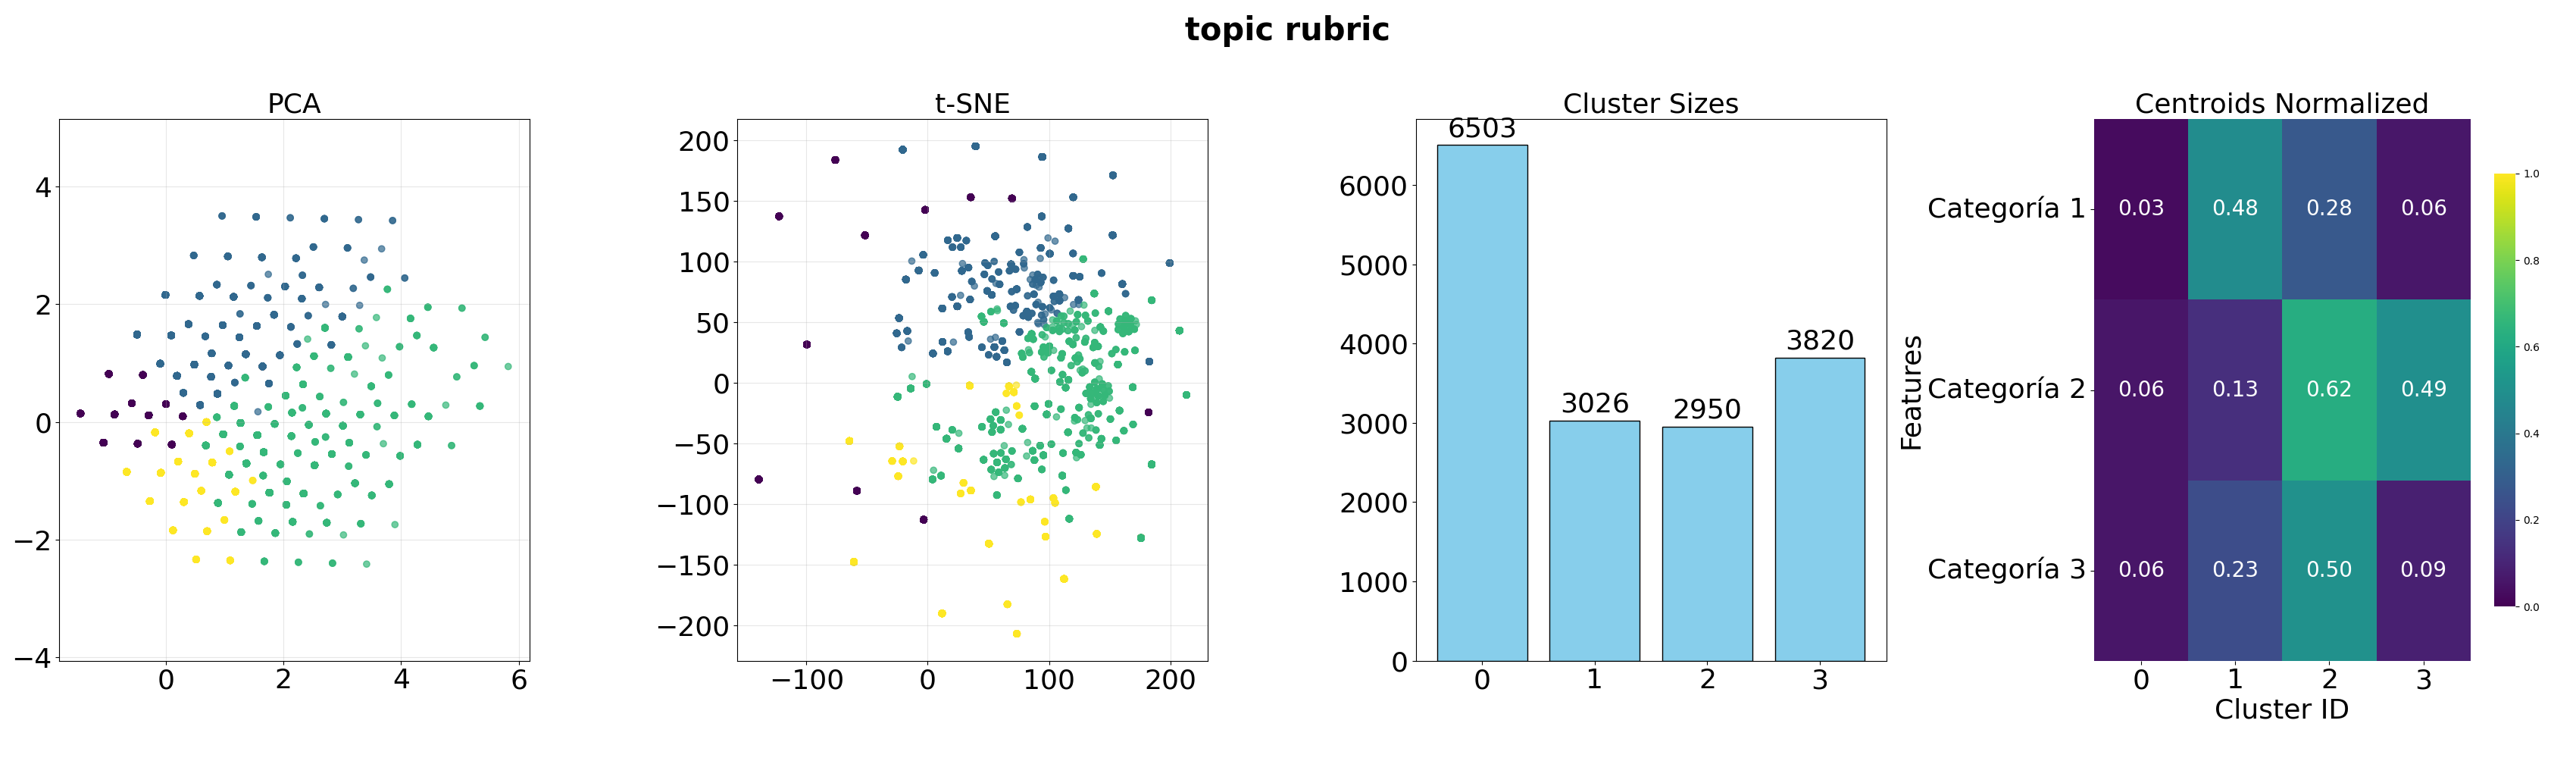
\includegraphics[width=\textwidth]{images/topic_rubric.png}
    \caption{Topic Rubric analysis.}
    \label{fig:topic_rubric}
\end{figure}

% 4: Topic Binary
\begin{figure}[htbp]
    \centering
    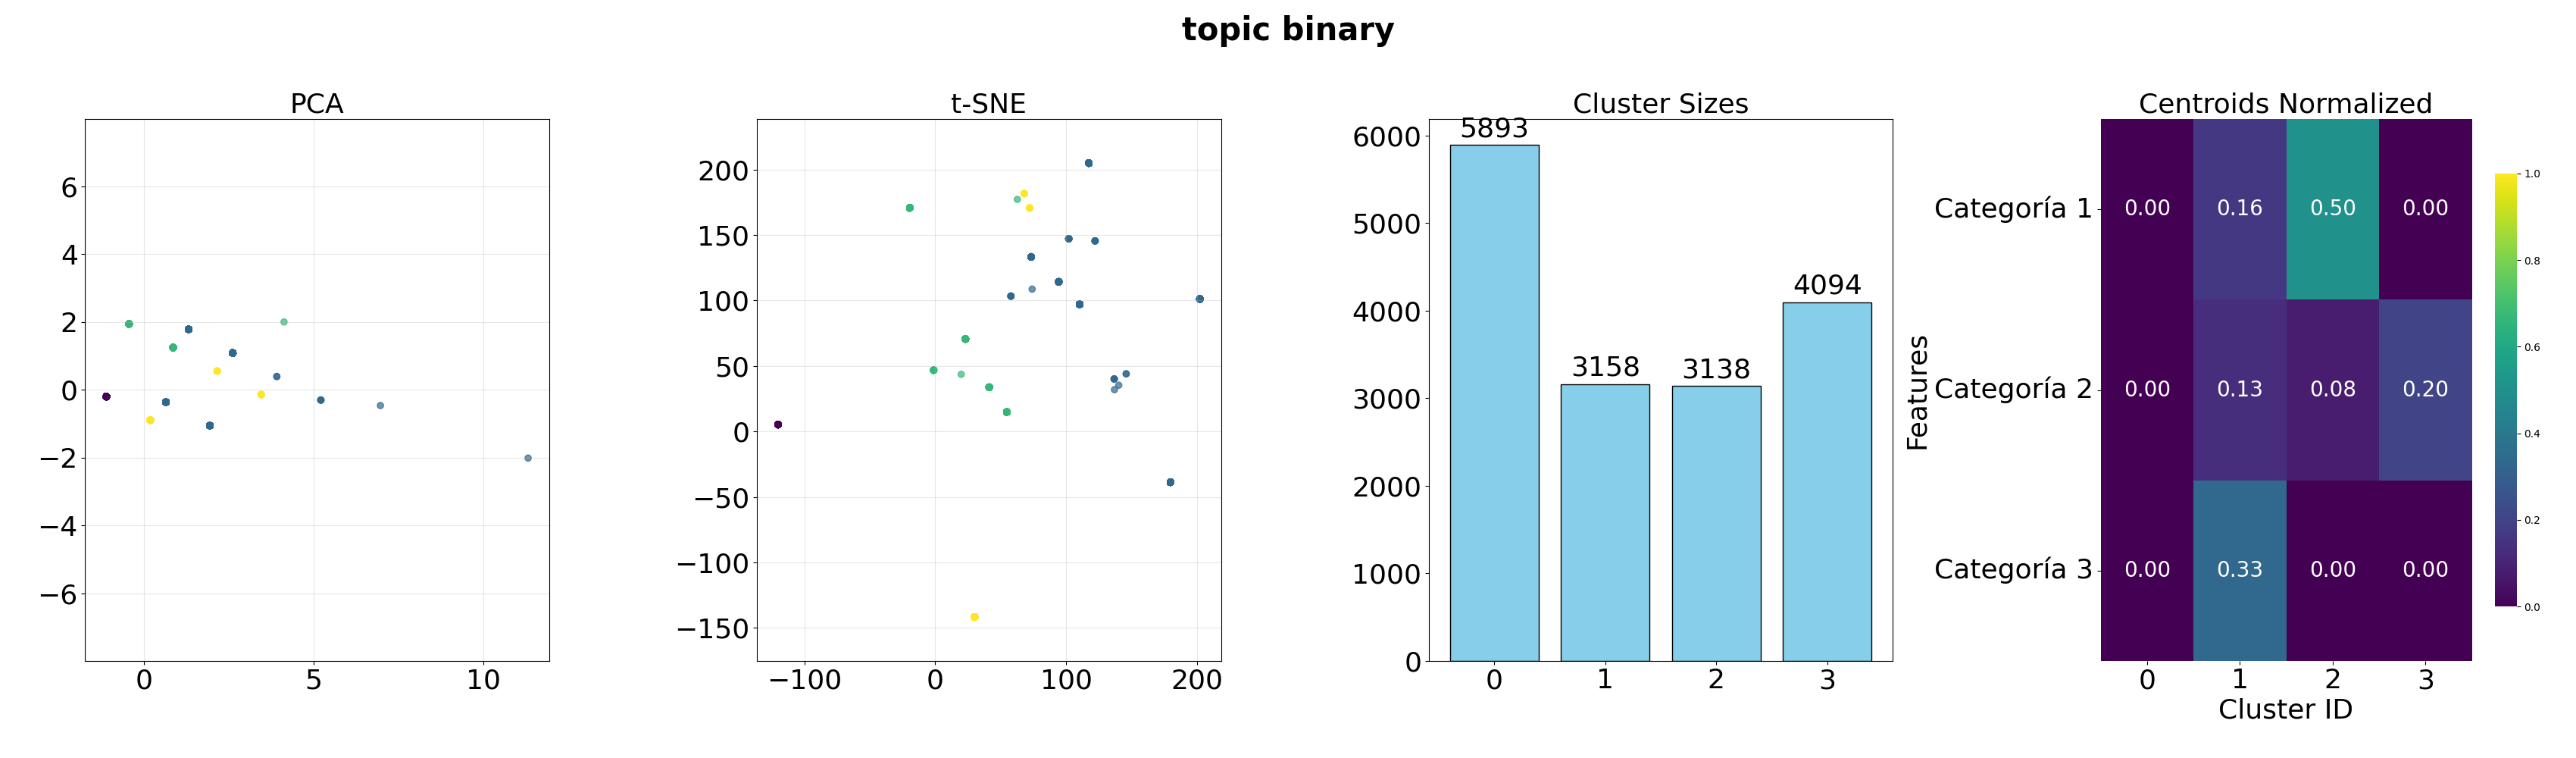
\includegraphics[width=\textwidth]{images/topic_binary.png}
    \caption{Topic Binary analysis.}
    \label{fig:topic_binary}
\end{figure}

% 5: Subtopic Rubric
\begin{figure}[htbp]
    \centering
    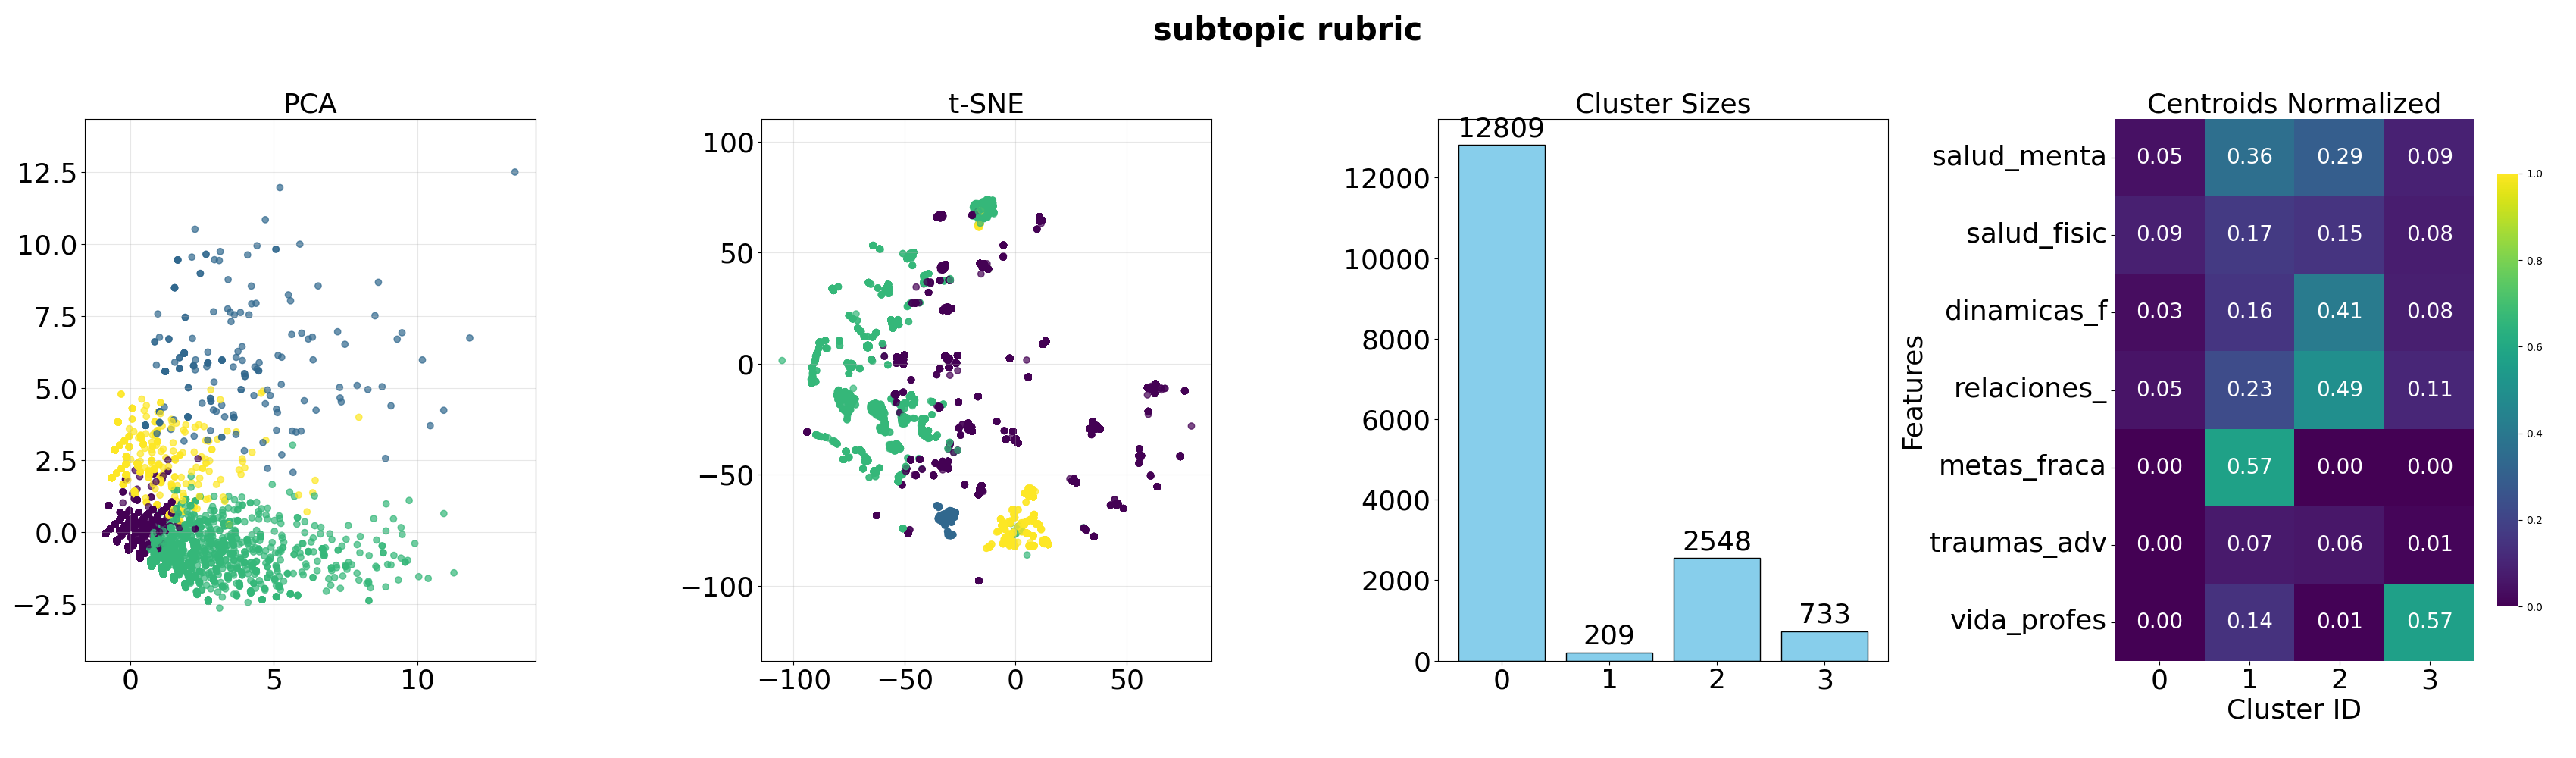
\includegraphics[width=\textwidth]{images/subtopic_rubric.png}
    \caption{Subtopic Rubric results.}
    \label{fig:subtopic_rubric}
\end{figure}

% 6: Subtopic Binary
\begin{figure}[htbp]
    \centering
    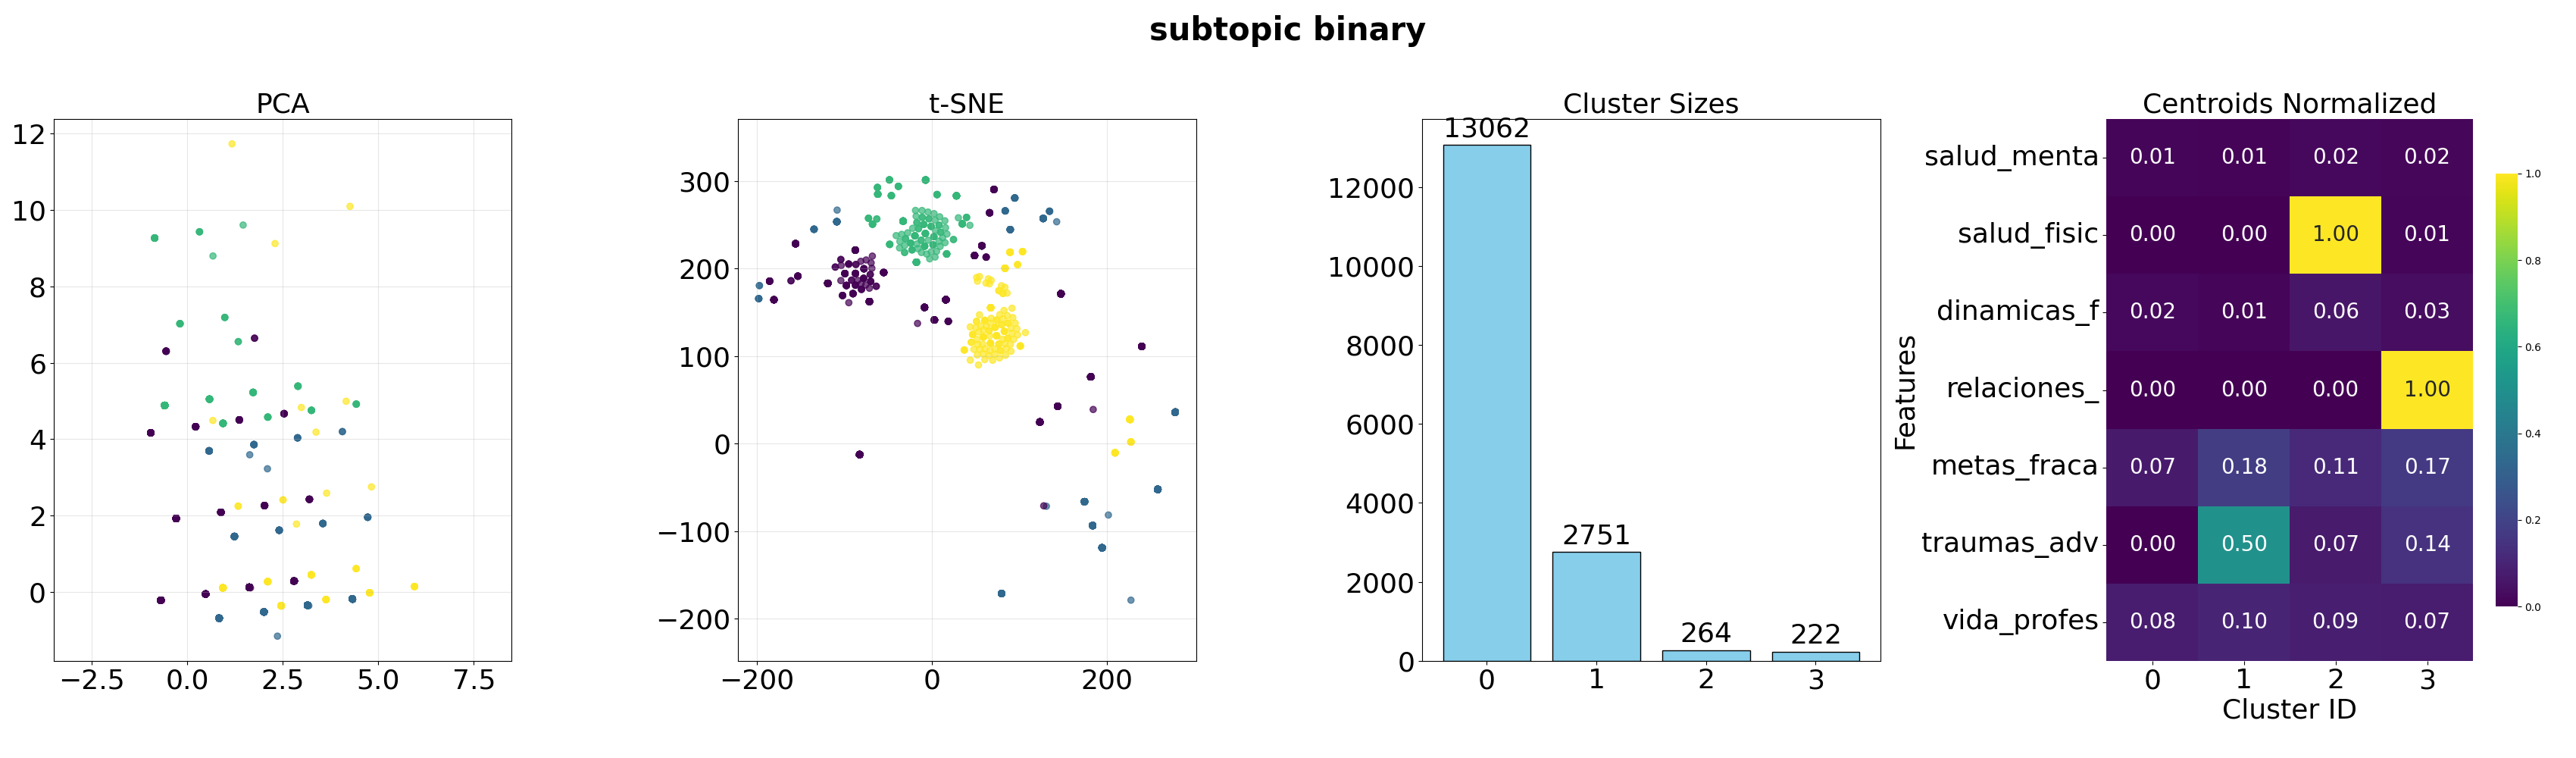
\includegraphics[width=\textwidth]{images/subtopic_binary.png}
    \caption{Subtopic Binary results.}
    \label{fig:subtopic_binary}
\end{figure}

Beyond the characterization of thematic clusters, a comprehensive review combining automated intensity scores and manual qualitative spot-checks suggests that approximately one-third of the final dataset (roughly 5,400 out of 16,301 sessions) constitutes true non-disclosure interactions. These sessions are primarily composed of phatic communication, greetings, or purely functional exchanges where the user does not progress beyond the outermost ``cliché" layer of the SPT. 

The identification of this significant volume of low-intimacy data provides a final empirical justification for our $3+1$ clustering strategy. By allowing the residual cluster to absorb this large proportion of non-revealing sessions, the architecture prevents the dilution of the primary behavioral profiles ($C_1$, $C_2$, and $C_3$). This ensures that the identified patterns of health, interpersonal, and historical disclosure remain statistically robust and qualitatively representative of genuine intimate interactions, rather than being overshadowed by the high frequency of superficial conversational mass.


% \newpage